\documentclass[27pt, landscape]{tikzposter}
\geometry{paperwidth=36in,paperheight=48in}
\colorlet{backgroundcolor}{white}
\colorlet{framecolor}{gray!20}
\colorlet{titlefgcolor}{black}
\colorlet{titlebgcolor}{gray!20}
\colorlet{blocktitlebgcolor}{purple}
\colorlet{blocktitlefgcolor}{black}
\defineblockstyle{style}{titleleft}{\ifBlockHasTitle\draw[color=blocktitlebgcolor] (blocktitle.south west) -- (blocktitle.south east);\fi}
\usepackage{lipsum}
\usepackage{tikz,lipsum,lmodern}
\usepackage[most]{tcolorbox}

\usepackage{fullpage}
\usepackage{enumitem}
\usepackage{lineno}
\usepackage[b]{esvect}
\usepackage[dvipsnames]{xcolor}
\usepackage{tikz}
\usepackage{caption}
\usepackage{subcaption}
\usepackage[font=footnotesize,labelfont=bf]{caption}
\usetikzlibrary{shapes.multipart,shapes.geometric,topaths,calc, positioning, decorations.pathreplacing, calligraphy}
\usepackage{epsfig}
\usepackage{amsfonts}
\usepackage{amssymb}
\usepackage{amstext}
\usepackage{amsmath}
\usepackage{xspace}
\usepackage{theorem}
\usepackage{xcolor}
\usepackage{color}
\usepackage{graphicx}
\usepackage{ifthen}
\usepackage{hyperref}
\usepackage[T1]{fontenc}
\usetikzlibrary{shapes,arrows}
\usepackage{multicol}

\newenvironment{proof}{{\bf Proof:  }}{\hfill\rule{2mm}{2mm}}
\newenvironment{proofof}[1]{{\bf Proof of #1:  }}{\hfill\rule{2mm}{2mm}}
\newenvironment{proofofnobox}[1]{{\bf#1:  }}{}
\newenvironment{example}{{\bf Example:  }}{\hfill\rule{2mm}{2mm}}


\newtheorem{theorem}{Theorem}
\newtheorem{lemma}[theorem]{Lemma}
\newtheorem{prop}[theorem]{Proposition}
\newtheorem{claim}[theorem]{Claim}
\newtheorem{corollary}[theorem]{Corollary}
\newtheorem{definition}[theorem]{Definition}
\newtheorem{problem}[theorem]{Problem}
\newtheorem{fact}[theorem]{Fact}
\newtheorem{conj}[theorem]{Conjecture}

\usepackage[backend=bibtex,isbn=false,url=false]{biblatex}


% math notation
\newcommand{\sq}{~\square~}
\newcommand{\F}{{\cal F}}
\newcommand{\lcm}{\text{lcm}}
\newcommand{\vvdots}[3][2]{\node[circle,fill,inner sep=1pt] at (#2 , #3)(a){};\node [below=3mm of a, circle,fill,inner sep=1pt]{};\node [above=3mm of a, circle,fill,inner sep=1pt]{}}

\title{Decompositions of Cartesian Products of Cycles}
\author{Moriah Aberle, Sarah Gold, Rivkah Moshe}
\institute{Denison University, Haverford College, Boston University \\\vspace{.5cm} Advisor: David Offner, Carnegie Mellon University}

\addbibresource{references.bib}


\begin{document}
\thispagestyle{empty} 
\useblockstyle{style}
\definetitlestyle{style}{width=36in}{\begin{scope}
\filldraw[gray!20]
(-90,\titleposbottom-25) rectangle (90,\titlepostop+30);
\end{scope}}
\usetitlestyle{style}
\maketitle
\node[anchor=west, xshift=8cm] at (TP@title.west) {
\includegraphics[width=10cm]{cmulogo.png}};
\node[anchor=east, xshift=-4cm] at (TP@title.east) {\includegraphics[width=16cm]{suamilogo.png}};


\begin{columns}[t]
    \column{0.25}
    \block{Graph Decompositions}{
    \begin{definition}[Graph]
        A \emph{graph} $G$ is a set of vertices $V(G)$ along with a set of edges $E(G)$ where each edge ``connects'' two vertices.
    \end{definition}
    
    \begin{definition}[Cycle]
        A \emph{cycle} of length $k$, denoted $C_k$ has $k$ vertices, ordered cyclically, with edges between consecutive vertices. 
    \end{definition}
    
    \textbf{Example:} Two representations of $C_6$.
    
    \begin{center}
        \begin{tikzpicture}[scale=1.2]
            \draw [ultra thick, -] (2,0) -- (0,1) -- (0,3) -- (2,4) -- (4,3) -- (4,1) -- (2,0);
            \node[shape=circle, draw=black, fill=white] at (2,0){1};
            \node[shape=circle, draw=black, fill=white] at (0,1){2};
            \node[shape=circle, draw=black, fill=white] at (0,3){3};
            \node[shape=circle, draw=black, fill=white] at (2,4){4};
            \node[shape=circle, draw=black, fill=white] at (4,3){5};
            \node[shape=circle, draw=black, fill=white] at (4,1){6};
            
            
            %\draw [-latex, ultra thick] (4.75,2) -- (6.25,2);
            \large{\node at (6,2) {$=$};}
            
            \draw [ultra thick, -] (7, 2) -- (19, 2);
            \foreach \i\j in {8/1,10/2,12/3,14/4,16/5,18/6}{
                \node[shape=circle, minimum size=0.5cm, draw=black, fill=white] at (\i,2){\j};
            }
        \end{tikzpicture}
    \end{center}
    
    \begin{definition}[Cartesian product]
        The \emph{Cartesian product} of two graphs $G$ and $H$, written $G \sq H$, is the graph with vertex set $V(G) \times V(H)$, where an edge $e = (u,v)  (u', v') \in E(G\sq H)$ if $u = u'$ and $vv' \in E(H)$, or if $v = v'$ and $uu' \in E(G)$.
    \end{definition}
    
    \begin{definition}[Decomposition]
        A \emph{decomposition} of a graph is a partition of the edges of the graph into copies of a fixed subgraph.
    \end{definition}
    
    \textbf{Example:} $C_4 \sq C_6$ decomposed into copies of $C_4$ (left) and $C_{24}$ (right).
    \begin{center}
        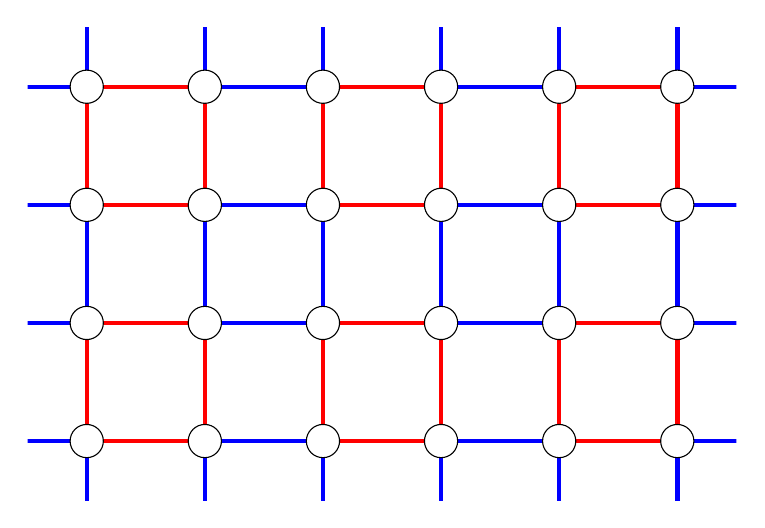
\begin{tikzpicture}[scale=1.5, transform shape]
            \clip (-0.5,-0.5) rectangle (5.5,3.5);
          
            \foreach \i in {0,2,...,6}{\foreach \j in {0,2,...,4}{
                \draw [ultra thick, -, color=red] (\i, \j) -- (\i+1, \j) -- (\i+1, \j+1) -- (\i, \j+1) -- (\i, \j);
            }}
          
            \foreach \i in {-1,1,...,5}{\foreach \j in {-1,1,...,5}{
                \draw [ultra thick, -, color=blue] (\i, \j) -- (\i+1, \j) -- (\i+1, \j+1) -- (\i, \j+1) -- (\i, \j);
            }}
          
            \foreach \i in {0,1,...,5}{\foreach \j in {0,1,2,3}{
                \filldraw[fill=white, draw=black] (\i, \j) circle (4pt);
            }}
        \end{tikzpicture} \hspace{3cm}
        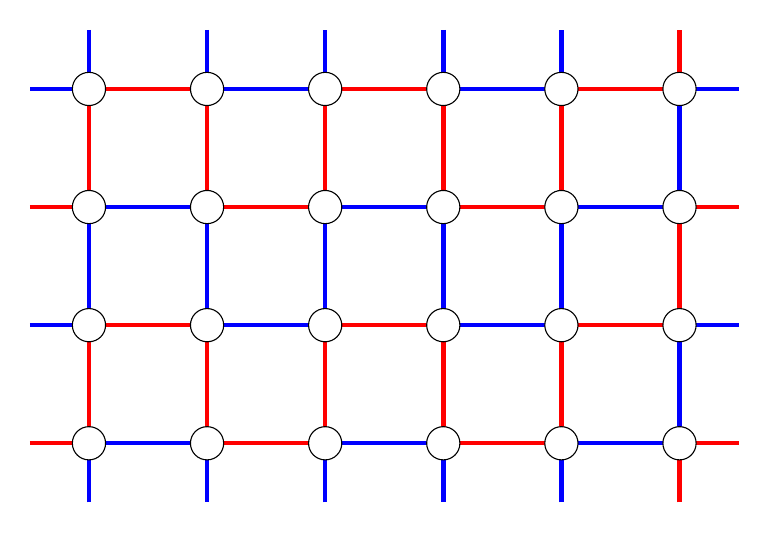
\begin{tikzpicture}[scale=1.5]
            \foreach \j\i in {0/red,1/blue}{
                \draw [ultra thick, -, color=\i] (6.5, \j) -- (7,\j) -- (7,\j+1) -- (8,\j+1) -- (8,\j) -- (9,\j) -- (9,\j+1) -- (10,\j+1) -- (10,\j) -- (11,\j) -- (11,\j+1) -- (12,\j+1) -- (12,\j+2) -- (12.5,\j+2);
            }
            \draw [ultra thick, -, color=red] (6.5, 2) -- (7,2) -- (7,3) -- (8,3) -- (8,2) -- (9,2) -- (9,3) -- (10,3) -- (10,2) -- (11,2) -- (11,3) -- (12,3) -- (12,3.5);
            \draw [ultra thick, -, color=red] (12,-0.5) -- (12,0) -- (12.5,0);
            \foreach \i in {7,9}{
                \draw [ultra thick, -, color=blue] (\i, -0.5) -- (\i, 0) -- (\i+1, 0) -- (\i+1, -0.5);
            }
            \foreach \i in {8,10}{
                \draw [ultra thick, -, color=blue] (\i, 3.5) -- (\i, 3) -- (\i+1, 3) -- (\i+1, 3.5);
            }
            \draw [ultra thick, -, color=blue] (11,-0.5) -- (11,0) -- (12,0) -- (12,1) -- (12.5,1);
            \draw [ultra thick, -, color=blue] (7,3.5) -- (7,3) -- (6.5,3);
            
            
            \foreach \i in {7,8,...,12}{\foreach \j in {0,1,2,3}{
                \filldraw[fill=white, draw=black] (\i, \j) circle (4pt);
            }}
    \end{tikzpicture}
    \end{center}
    
    \textbf{Example:} $C_8 \sq C_{18}$ decomposed into copies of $C_{96}$.
    \begin{center}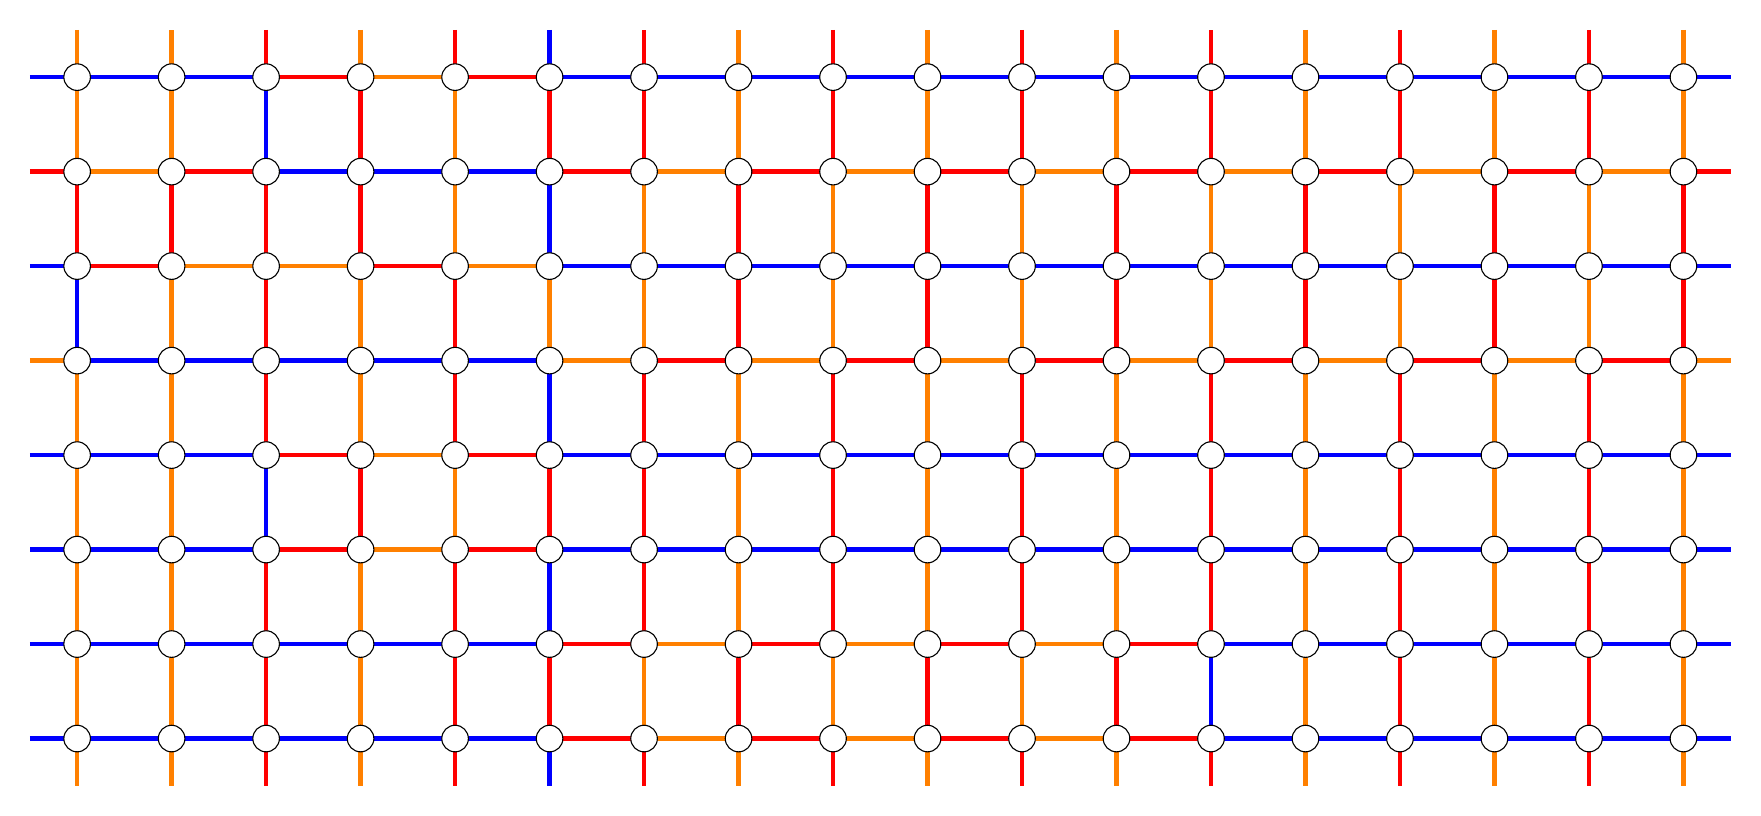
\begin{tikzpicture} [scale=1.2]
%A Block
    \draw[blue, ultra thick] (-.5, 0) -- (2, 0) -- (2, -1) -- (5, -1) -- (5, -2) -- (5.5, -2); \draw[blue, ultra thick] (-.5, -2) -- (0, -2) -- (0, -3) -- (5, -3) -- (5, -4) -- (5.5, -4); \draw[blue, ultra thick] (5, .5) -- (5, 0) -- (5.5, 0); \draw[blue, ultra thick] (5.5, -5) -- (5, -5) -- (5, -5.5); \draw[blue, ultra thick] (-.5, -4) -- (2, -4) -- (2, -5) -- (-.5, -5);
    \draw[orange, ultra thick] (0, .5) -- (0, -1) -- (1, -1) -- (1, .5); \draw[orange, ultra thick] (3, .5) -- (3, 0) -- (4, 0) -- (4, -2) -- (5, -2) -- (5, -3) -- (5.5, -3); \draw[orange, ultra thick] (-.5, -3) -- (0, -3) -- (0, -5.5); \draw[orange, ultra thick] (1, -5.5)  -- (1, -2) -- (3, -2) -- (3, -4) -- (4, -4) -- (4, -5) -- (3, -5) -- (3, -5.5);
    \draw[red, ultra thick] (-.5, -1) -- (0, -1) -- (0, -2) -- (1, -2) -- (1, -1) -- (2, -1) -- (2, -4) -- (3, -4) -- (3, -5) -- (2, -5) -- (2, -5.5); \draw[red, ultra thick] (2, .5) -- (2, 0) -- (3, 0) -- (3, -2) -- (4, -2) -- (4, -4) -- (5, -4) -- (5, -5) -- (4, -5) -- (4, -5.5); \draw[red, ultra thick] (4, .5) -- (4, 0) -- (5, 0) -- (5, -1) -- (5.5, -1);
    \foreach \x in {0, 1, ..., 5}{\foreach \y in {0, -1, ..., -5}{\filldraw[draw=black, fill=white] (\x, \y) circle (4pt);}}
%B Block 1
    \draw[blue, ultra thick] (6-0.5, 0) -- (12-0.5, 0); \draw[blue, ultra thick] (6-0.5, -2) -- (12-0.5, -2); \draw[blue, ultra thick] (6-0.5, -4) -- (12-0.5, -4); \draw[blue, ultra thick] (6-0.5, -5) -- (12-0.5, -5);
    \draw[red, ultra thick] (6-0.5, -1) -- (6.5-0.5, -1) -- (6.5-0.5, .5); \draw[red, ultra thick] (8.5-0.5, .5) -- (8.5-0.5, -1) -- (7.5-0.5, -1) -- (7.5-0.5, -3) -- (6.5-0.5, -3) -- (6.5-0.5, -5.5); \draw[red, ultra thick] (10.5-0.5, .5) -- (10.5-0.5, -1) -- (9.5-0.5, -1) -- (9.5-0.5, -3) -- (8.5-0.5, -3) -- (8.5-0.5, -5.5); \draw[red, ultra thick] (12-0.5, -1) -- (11.5-0.5, -1) -- (11.5-0.5, -3) -- (10.5-0.5, -3) -- (10.5-0.5, -5.5);
    \draw[orange, ultra thick] (7.5-0.5, .5) -- (7.5-0.5, -1) -- (6.5-0.5, -1) -- (6.5-0.5, -3) -- (6-0.5, -3); \draw[orange, ultra thick] (9.5-0.5, .5) -- (9.5-0.5, -1) -- (8.5-0.5, -1) -- (8.5-0.5, -3) -- (7.5-0.5, -3) -- (7.5-0.5, -5.5); \draw[orange, ultra thick] (11.5-0.5, .5) -- (11.5-0.5, -1) -- (10.5-0.5, -1) -- (10.5-0.5, -3) -- (9.5-0.5, -3) -- (9.5-0.5, -5.5); \draw[orange, ultra thick] (12-0.5, -3) -- (11.5-0.5, -3) -- (11.5-0.5, -5.5);
    \foreach \x in {6.5, 7.5, 8.5, 9.5, 10.5, 11.5}{\foreach \y in {0, -1, ..., -5}{\filldraw[draw=black, fill=white] (\x-0.5, \y) circle (4pt);}}
    %B Block 2
    \draw[blue, ultra thick] (6+5.5, 0) -- (12+5.5, 0); \draw[blue, ultra thick] (6+5.5, -2) -- (12+5.5, -2); \draw[blue, ultra thick] (6+5.5, -4) -- (12+5.5, -4); \draw[blue, ultra thick] (6+5.5, -5) -- (12+5.5, -5);
    \draw[red, ultra thick] (6+5.5, -1) -- (6.5+5.5, -1) -- (6.5+5.5, .5); \draw[red, ultra thick] (8.5+5.5, .5) -- (8.5+5.5, -1) -- (7.5+5.5, -1) -- (7.5+5.5, -3) -- (6.5+5.5, -3) -- (6.5+5.5, -5.5); \draw[red, ultra thick] (10.5+5.5, .5) -- (10.5+5.5, -1) -- (9.5+5.5, -1) -- (9.5+5.5, -3) -- (8.5+5.5, -3) -- (8.5+5.5, -5.5); \draw[red, ultra thick] (12+5.5, -1) -- (11.5+5.5, -1) -- (11.5+5.5, -3) -- (10.5+5.5, -3) -- (10.5+5.5, -5.5);
    \draw[orange, ultra thick] (7.5+5.5, .5) -- (7.5+5.5, -1) -- (6.5+5.5, -1) -- (6.5+5.5, -3) -- (6+5.5, -3); \draw[orange, ultra thick] (9.5+5.5, .5) -- (9.5+5.5, -1) -- (8.5+5.5, -1) -- (8.5+5.5, -3) -- (7.5+5.5, -3) -- (7.5+5.5, -5.5); \draw[orange, ultra thick] (11.5+5.5, .5) -- (11.5+5.5, -1) -- (10.5+5.5, -1) -- (10.5+5.5, -3) -- (9.5+5.5, -3) -- (9.5+5.5, -5.5); \draw[orange, ultra thick] (12+5.5, -3) -- (11.5+5.5, -3) -- (11.5+5.5, -5.5);
    \foreach \x in {6.5, 7.5, 8.5, 9.5, 10.5, 11.5}{\foreach \y in {0, -1, ..., -5}{\filldraw[draw=black, fill=white] (\x+5.5, \y) circle (4pt);}}
%C Block
    \draw[blue, ultra thick] (-.5, -6.5+0.5) -- (5, -6.5+0.5) -- (5, -6+0.5); \draw[blue, ultra thick] (-.5, -7.5+0.5) -- (5, -7.5+0.5) -- (5, -8+0.5); %\draw[blue, ultra thick] (12, -6.5+0.5) -- (10.5, -6.5+0.5) -- (10.5, -7.5+0.5) -- (12, -7.5+0.5); 
    \draw [blue, ultra thick] (17.5,-6) -- (12,-6) -- (12,-7) -- (17.5,-7);
    \draw[orange, ultra thick] (0, -6+0.5) -- (0, -8+0.5); \draw[orange, ultra thick] (1, -6+0.5) -- (1, -8+0.5); \draw[orange, ultra thick] (3, -6+0.5) -- (3, -8+0.5); 
    \foreach \i in {6,8,...,12}{
        \draw [red, ultra thick] (\i, -5.5) -- (\i, -6) -- (\i-1, -6) -- (\i-1, -7) -- (\i, -7) -- (\i, -7.5);
    }
    \foreach \i in {7,9,11}{
        \draw [orange, ultra thick] (\i, -5.5) -- (\i, -6) -- (\i-1, -6) -- (\i-1, -7) -- (\i, -7) -- (\i, -7.5);
    }
    \foreach \i in {13,15,17}{
        \draw [orange, ultra thick] (\i, -5.5) -- (\i, -7.5);
    }
    \foreach \i in {14,16}{
        \draw [red, ultra thick] (\i, -5.5) -- (\i, -7.5);
    }
    %\draw[orange, ultra thick] (7.5, -6+0.5) -- (7.5, -6.5+0.5) -- (6.5, -6.5+0.5) -- (6.5, -7.5+0.5) -- (7.5, -7.5+0.5) -- (7.5, -8+0.5); \draw[orange, ultra thick] (9.5, -6+0.5) -- (9.5, -6.5+0.5) -- (8.5, -6.5+0.5) -- (8.5, -7.5+0.5) -- (9.5, -7.5+0.5) -- (9.5, -8+0.5); \draw[orange, ultra thick] (11.5, -6+0.5) -- (11.5, -8+0.5);
    \draw[red, ultra thick] (2, -6+0.5) -- (2, -8+0.5);\draw[red, ultra thick] (4, -6+0.5) -- (4, -8+0.5); %\draw[red, ultra thick] (6.5, -6+0.5) -- (6.5, -6.5+0.5) -- (5, -6.5+0.5) -- (5, -7.5+0.5) -- (6.5, -7.5+0.5) -- (6.5, -8+0.5); \draw[red, ultra thick] (8.5, -6+0.5) -- (8.5, -6.5+0.5) -- (7.5, -6.5+0.5) -- (7.5, -7.5+0.5) -- (8.5, -7.5+0.5) -- (8.5, -8+0.5);\draw[red, ultra thick] (10.5, -6+0.5) -- (10.5, -6.5+0.5) -- (9.5, -6.5+0.5) -- (9.5, -7.5+0.5) -- (10.5, -7.5+0.5) -- (10.5, -8+0.5);
    \foreach \x in {0, 1,...,17}{\foreach \y in {-6.5, -7.5}{\filldraw[draw=black, fill=white] (\x, \y+0.5) circle (4pt);}}
\end{tikzpicture}\end{center}
    
    \textbf{Motivating Theorem} 
    \textbf{(Kotzig, 1973)}\\ \textit{$C_{mn}$ decomposes $C_m \sq C_n$}. 
    
    \begin{tcolorbox}[colback=red!5!white,colframe=red!65!black,title=Research Questions:]
    \begin{itemize}
        \item Given $m$ and $n$, what cycles $C_k$ decompose $C_m \sq C_n$?
        \item Given a cycle length $k$, what Cartesian products $C_m \sq C_n$ does $C_k$ decompose?
    \end{itemize}
\end{tcolorbox}
    
    \begin{theorem}[Divisibility Criterion]
        If $C_k$ decomposes $C_m \sq C_n$, then $k$ divides the number of edges, $2\cdot m \cdot n$.
    \end{theorem}
    \begin{theorem}
        $C_4$ decomposes $C_m \sq C_n$ $\iff$ $2 \mid m,n$.
    \end{theorem}
    }
     
    

    
    \column{0.25}
    \block{Decomposing where $4 \mid m$ and $4 \mid n$}{
    \begin{theorem}
        Let $G = C_{m} \sq C_{n}$ where $4 \mid m$ and $4 \mid n$. If $4 \mid k$ and $k \mid mn$, then $C_k$ decomposes $G$.
    \end{theorem}
    
    \textbf{Proof:} Cycle combination operation:
    
    \begin{center}
        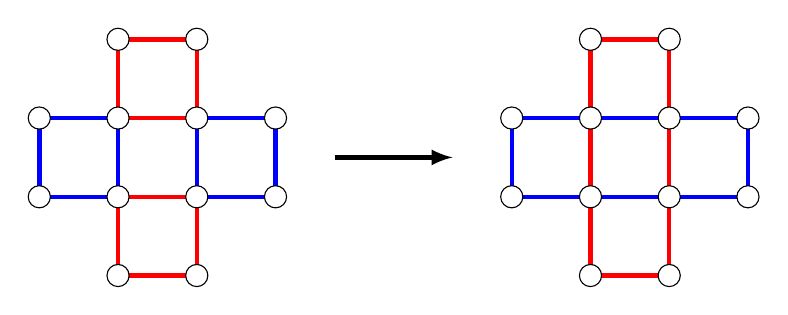
\begin{tikzpicture}
            \draw [ultra thick, -, color=red] (0,0) -- (0, 1) -- (1,1) -- (1, 0) -- (0,0);
            \draw [ultra thick, -, color=red] (0, 2) -- (0, 3) -- (1, 3) -- (1, 2) -- (0, 2);
            \draw [ultra thick, -, color=blue] (-1, 1) -- (-1, 2) -- (0, 2) -- (0, 1) -- (-1, 1);
            \draw [ultra thick, -, color=blue] (1, 1) -- (1, 2) -- (2, 2) -- (2, 1) -- (1, 1);
                
            \foreach \i in {0, 1}{\foreach \j in {1, 2}{\filldraw[fill=white, draw=black] (\i, \j) circle (4pt);}}    
            \foreach \j in {1, 2}{\filldraw[fill=white, draw=black] (-1, \j) circle (4pt);}
            \foreach \j in {1, 2}{\filldraw[fill=white, draw=black] (2, \j) circle (4pt);}
            \foreach \i in {0, 1}{\filldraw[fill=white, draw=black] (\i, 3) circle (4pt);}
            \foreach \i in {0, 1}{\filldraw[fill=white, draw=black] (\i, 0) circle (4pt);}
            
            \draw [ultra thick, -, color=red] (6,0) -- (6, 3) -- (7, 3) -- (7, 0) -- (6, 0);
            \draw [ultra thick, -, color=blue] (5, 2) -- (8, 2) -- (8, 1) -- (5, 1) -- (5, 2);
                
            \foreach \i in {6, 7}{\foreach \j in {1, 2}{\filldraw[fill=white, draw=black] (\i, \j) circle (4pt);}}
            \foreach \j in {1, 2}{\filldraw[fill=white, draw=black] (5, \j) circle (4pt);}
            \foreach \j in {1, 2}{\filldraw[fill=white, draw=black] (8, \j) circle (4pt);}
            \foreach \i in {6, 7}{\filldraw[fill=white, draw=black] (\i, 3) circle (4pt);}
            \foreach \i in {6, 7}{\filldraw[fill=white, draw=black] (\i, 0) circle (4pt);}
            
            \draw [-latex, ultra thick] (2.75,1.5) -- (4.25,1.5);
                
        \end{tikzpicture}
        \label{fig:zoomedInCycleCombo}
    \end{center}
    
    From a decomposition of $C_n \sq C_m$ into copies of $C_4$, number selected locations where cycle combination operation can be applied, and perform operation. Demonstrated with a decomposition of $C_{12} \sq C_8$ into copies of $C_{12}$.
    
    
    \begin{center}
        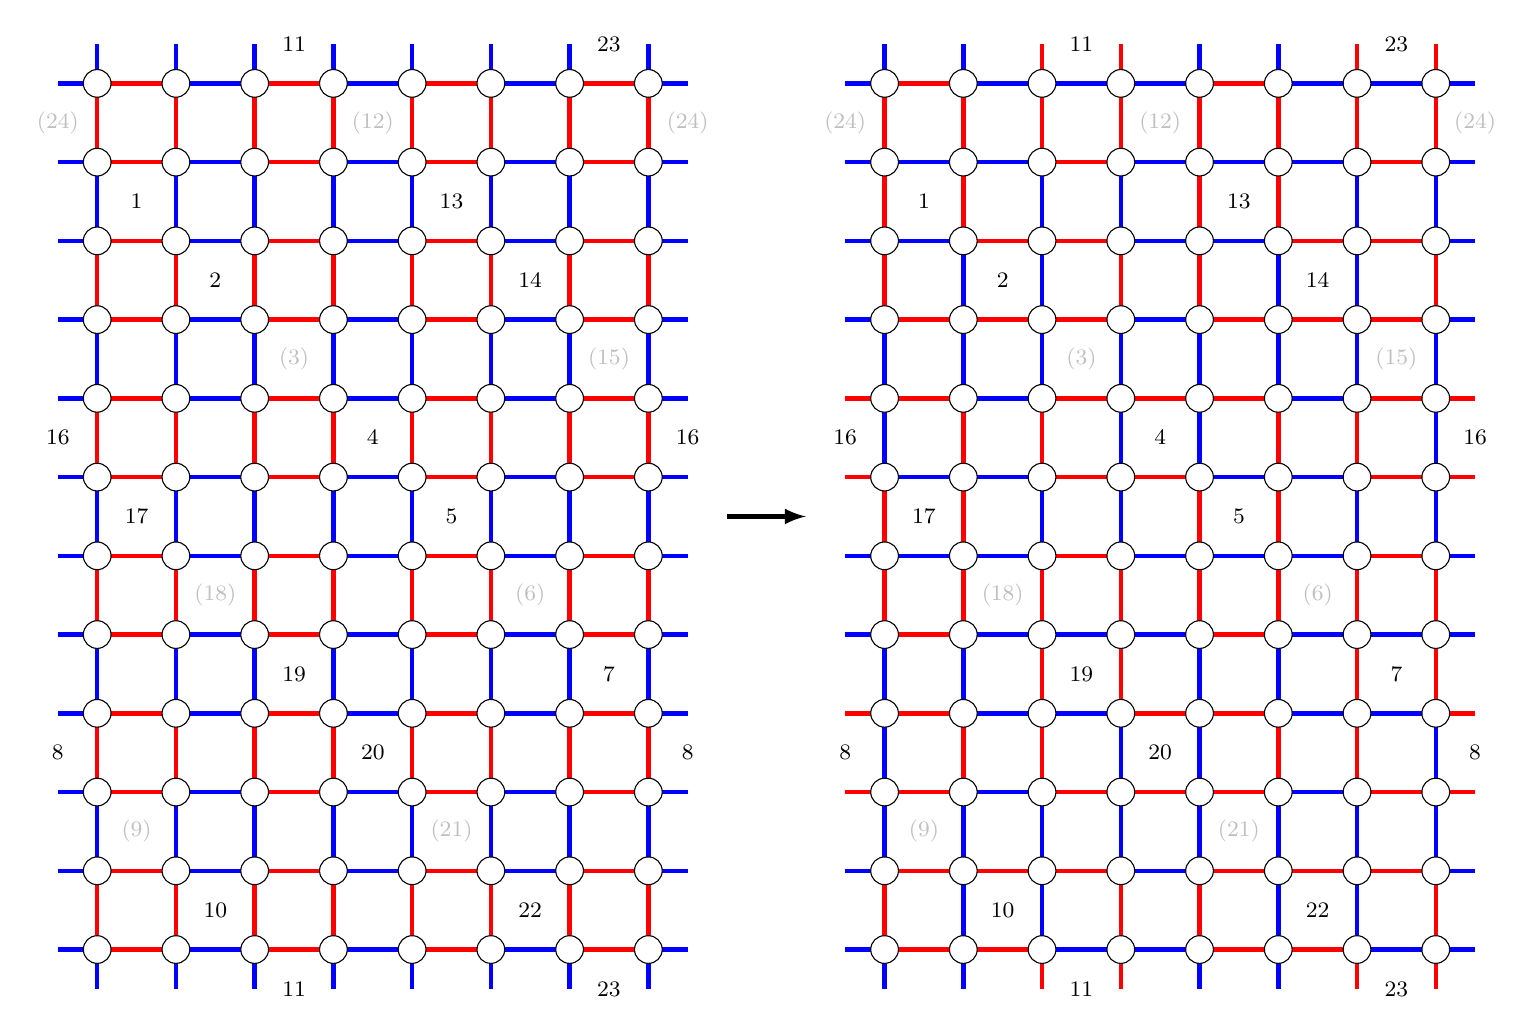
\begin{tikzpicture}
            \foreach \i in {0,2,...,6}{\foreach \j in {0,2,...,10}{
                \draw [ultra thick, -, color=red] (\i, \j) -- (\i+1, \j) -- (\i+1, \j+1) -- (\i, \j+1) -- (\i, \j);
            }}
            \foreach \i in {1,3,5}{\foreach \j in {1,3,...,9}{
                \draw [ultra thick, -, color=blue] (\i, \j) -- (\i+1, \j) -- (\i+1, \j+1) -- (\i, \j+1)  -- (\i, \j);
            }
                \draw [ultra thick, -, color=blue] (\i, 11.5) -- (\i, 11) -- (\i+1, 11) -- (\i+1, 11.5);
                \draw [ultra thick, -, color=blue] (\i, -0.5) -- (\i, 0) -- (\i+1, 0) -- (\i+1, -0.5);
            }
            \foreach \j in {1,3,...,9}{
                \draw [ultra thick, -, color=blue] (-0.5, \j) -- (0, \j) -- (0, \j+1) -- (-0.5, \j+1);
                \draw [ultra thick, -, color=blue] (7.5, \j) -- (7, \j) -- (7, \j+1) -- (7.5, \j+1);
            }
            \draw [ultra thick, -, color=blue] (-0.5, 0) -- (0,0) -- (0, -0.5);
            \draw [ultra thick, -, color=blue] (-0.5, 11) -- (0,11) -- (0, 11.5);
            \draw [ultra thick, -, color=blue] (7.5, 11) -- (7, 11) -- (7, 11.5);
            \draw [ultra thick, -, color=blue] (7.5, 0) -- (7, 0) -- (7, -0.5);
            
            \foreach \i in {1,2,...,8}{
                \node [align=center] at (\i-0.5, 10.5-\i) {\ifthenelse{\i=3 \OR \i=6}{\textcolor{gray!50}{\footnotesize $(\i)$}}{\footnotesize $\i$}};
            }   
            \foreach \i in {8,9,...,11}{
                \node [align=center] at (\i-8.5, 10.5-\i) {\ifthenelse{\i=9}{\textcolor{gray!50}{\footnotesize $(\i)$}}{\footnotesize $\i$}};
            }
            \foreach \i in {11,12,...,16}{
                \node [align=center] at (\i-8.5, 22.5-\i) {\ifthenelse{\i=12 \OR \i=15}{\textcolor{gray!50}{\footnotesize $(\i)$}}{\footnotesize $\i$}};
            }
            \foreach \i in {16,17,...,23}{
                \node [align=center] at (\i-16.5, 22.5-\i) {\ifthenelse{\i=18 \OR \i=21}{\textcolor{gray!50}{\footnotesize $(\i)$}}{\footnotesize $\i$}};
            }
            \foreach \i in {23,24}{
                \node [align=center] at (\i-16.5, 34.5-\i) {\ifthenelse{\i=24}{\textcolor{gray!50}{\footnotesize $(\i)$}}{\footnotesize $\i$}};
            }
            \node [align=center] at (-0.5,10.5) {\textcolor{gray!50}{\footnotesize $(24)$}};

            \foreach \i in {0,1,...,7}{\foreach \j in {0,1,...,11}{\filldraw[fill=white, draw=black] (\i, \j) circle (5pt);}}
            
            % After Combination
            
            \foreach \i in {1,2,...,8}{
                \node [align=center] at (\i-0.5+10, 10.5-\i) {\ifthenelse{\i=3 \OR \i=6}{\textcolor{gray!50}{\footnotesize $(\i)$}}{\footnotesize $\i$}};
            }   
            \foreach \i in {8,9,...,11}{
                \node [align=center] at (\i-8.5+10, 10.5-\i) {\ifthenelse{\i=9}{\textcolor{gray!50}{\footnotesize $(\i)$}}{\footnotesize $\i$}};
            }
            \foreach \i in {11,12,...,16}{
                \node [align=center] at (\i-8.5+10, 22.5-\i) {\ifthenelse{\i=12 \OR \i=15}{\textcolor{gray!50}{\footnotesize $(\i)$}}{\footnotesize $\i$}};
            }
            \foreach \i in {16,17,...,23}{
                \node [align=center] at (\i-16.5+10, 22.5-\i) {\ifthenelse{\i=18 \OR \i=21}{\textcolor{gray!50}{\footnotesize $(\i)$}}{\footnotesize $\i$}};
            }
            \foreach \i in {23,24}{
                \node [align=center] at (\i-16.5+10, 34.5-\i) {\ifthenelse{\i=24}{\textcolor{gray!50}{\footnotesize $(\i)$}}{\footnotesize $\i$}};
            }
            \node [align=center] at (-0.5+10,10.5) {\textcolor{gray!50}{\footnotesize $(24)$}};
            
            \foreach \i in {10,14}{
                \draw [ultra thick, -, color=red] (\i,8) -- (\i+3,8) -- (\i+3,9) -- (\i+1,9) -- (\i+1,  11) -- (\i, 11) -- (\i, 8);
            }
            \draw [ultra thick, -, color=red] (9.5,7) -- (11,7) -- (11,4) -- (10,4) -- (10,6) -- (9.5,6);
            \draw [ultra thick, -, color=red] (12,7) -- (15,7) -- (15,4) -- (14,4) -- (14,6) -- (12,6) -- (12,7);
            \draw [ultra thick, -, color=red] (17.5,7) -- (16, 7) -- (16,6) -- (17.5, 6);
            \draw [ultra thick, -, color=red] (12,5) -- (13,5) -- (13,3) -- (15,3) -- (15,2) -- (12,2) -- (12,5);
            \draw [ultra thick, -, color=red] (17.5,2) -- (16,2) -- (16,5) -- (17,5) -- (17,3) -- (17.5,3);
            \draw [ultra thick, -, color=red] (9.5,3) -- (11, 3) -- (11,2) -- (9.5,2);
            \draw [ultra thick, -, color=red] (12,-0.5) -- (12,0) -- (10,0) -- (10,1) -- (13,1) -- (13,-0.5);
            \draw [ultra thick, -, color=red] (16,-0.5) -- (16,0) -- (14,0) -- (14,1) -- (17,1) -- (17,-0.5);
            \draw [ultra thick, -, color=red] (12,11.5) -- (12,10) -- (13,10) -- (13,11.5);
            \draw [ultra thick, -, color=red] (16,11.5) -- (16,10) -- (17,10) -- (17,11.5);
            
            \draw [ultra thick, -, color=blue] (9.5,10) -- (12,10) -- (12,7) -- (11,7) -- (11,9) -- (9.5,9);
            \draw [ultra thick, -, color=blue] (17.5,10) -- (17,10) -- (17,9) -- (17.5,9);
            \draw [ultra thick, -, color=blue] (13,10) -- (16,10) -- (16,7) -- (15,7) -- (15,9) -- (13,9) -- (13,10);
            \draw [ultra thick, -, color=blue] (13,8) -- (13,5) -- (16,5) -- (16,6) -- (14,6) -- (14,8) -- (13,8);
            \draw [ultra thick, -, color=blue] (17.5,8) -- (17,8) -- (17,5) -- (17.5,5);
            \draw [ultra thick, -, color=blue] (9.5,8) -- (10,8) -- (10,6) -- (12,6) -- (12,5) -- (9.5,5);
            \draw [ultra thick, -, color=blue] (11,4) -- (14,4) -- (14,1) -- (13,1) -- (13,3) -- (11,3) -- (11,4);
            \draw [ultra thick, -, color=blue] (17.5,4) -- (15,4) -- (15,3) -- (17,3) -- (17,1) -- (17.5,1);
            \draw [ultra thick, -, color=blue] (9.5,4) -- (10,4) -- (10,1) -- (9.5,1);
            \draw [ultra thick, -, color=blue] (11,-0.5) -- (11,2) -- (12,2) -- (12,0) -- (14,0) -- (14,-0.5);
            \draw [ultra thick, -, color=blue] (11,11.5) -- (11,11) -- (14,11) -- (14,11.5);
            \draw [ultra thick, -, color=blue] (15,-0.5) -- (15,2) -- (16,2) -- (16,0) -- (17.5,0);
            \draw [ultra thick, -, color=blue] (9.5,0) -- (10,0) -- (10,-0.5);
            \draw [ultra thick, -, color=blue] (10,11.5) -- (10,11) -- (9.5,11);
            \draw [ultra thick, -, color=blue] (17.5,11) -- (15,11) -- (15,11.5);
            
            \foreach \i in {0,1,...,7}{\foreach \j in {0,1,...,11}{\filldraw[fill=white, draw=black] (\i+10, \j) circle (5pt);}}
            
            \draw [-latex, ultra thick] (8,5.5) -- (9,5.5);
        \end{tikzpicture}
    \end{center}
    
    If $\gcd(m,n) \neq 2^i$, for some cycle lengths it is necessary to perform a second phase of the cycle combination operation. Shown below: decomposition of $C_{12} \sq C_{24}$ into copies of $C_{36}$.
    
    \begin{center}
    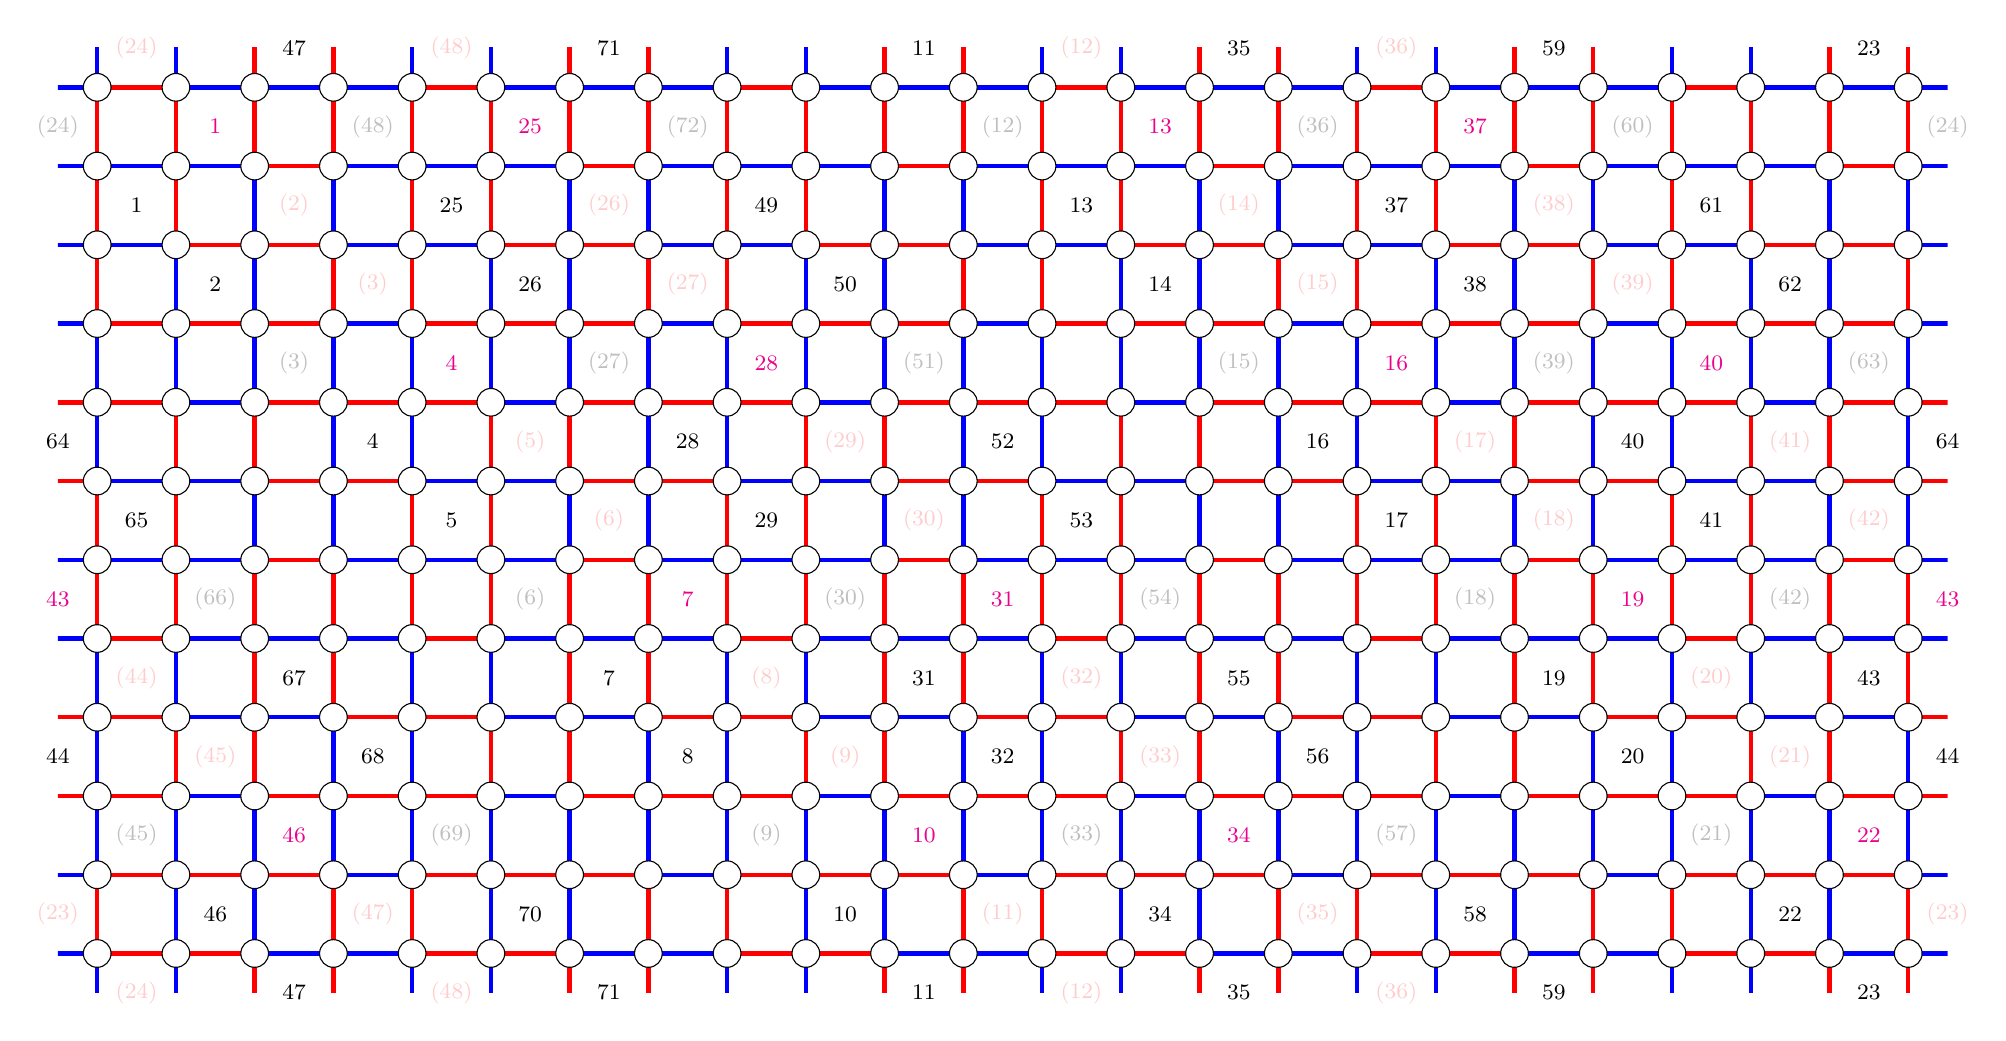
\begin{tikzpicture}
        \foreach \i in {1,2,...,11}{
            \node [align=center] at (\i-0.5, 10.5-\i) {\ifthenelse{\i=3 \OR \i=6 \OR \i=9}{\textcolor{gray!50}{\footnotesize $(\i)$}}{\footnotesize $\i$}};
        }
        \foreach \i in {11,12,...,23}{
            \node [align=center] at (\i-0.5, 10.5-\i+12) {\ifthenelse{\i=12 \OR \i=15 \OR \i=18 \OR \i=21}{\textcolor{gray!50}{\footnotesize $(\i)$}}{\footnotesize $\i$}};
        }
        \foreach \i in {23,24}{
            \node [align=center] at (\i-0.5, 10.5-\i+24) {\ifthenelse{\i=24}{\textcolor{gray!50}{\footnotesize $(\i)$}}{\footnotesize $\i$}};
        }
        \node [align=center] at (-0.5, 10.5) {\textcolor{gray!50}{\footnotesize $(24)$}};
        \foreach \i in {25,26,...,35}{
            \node [align=center] at (\i-0.5-20, 10.5-\i+24) {\ifthenelse{\i=27 \OR \i=30 \OR \i=33}{\textcolor{gray!50}{\footnotesize $(\i)$}}{\footnotesize $\i$}};
        }
        \foreach \i in {35,36,...,44}{
            \node [align=center] at (\i-0.5-20, 10.5-\i+36) {\ifthenelse{\i=36 \OR \i=39 \OR \i=42}{\textcolor{gray!50}{\footnotesize $(\i)$}}{\footnotesize $\i$}};
        }
        \foreach \i in {44,45,...,47}{
            \node [align=center] at (\i-0.5-44, 10.5-\i+36) {\ifthenelse{\i=45}{\textcolor{gray!50}{\footnotesize $(\i)$}}{\footnotesize $\i$}};
        }
        \node [align=center] at (2.5, 11.5) {\footnotesize $47$};
        \node [align=center] at (3.5, 10.5) {\textcolor{gray!50}{\footnotesize $(48)$}};
        
        \foreach \i in {49,50,...,59}{
            \node [align=center] at (\i-0.5-40, 10.5-\i+48) {\ifthenelse{\i=51 \OR \i=54 \OR \i=57}{\textcolor{gray!50}{\footnotesize $(\i)$}}{\footnotesize $\i$}};
        }
        \foreach \i in {59, 60,...,64}{
            \node [align=center] at (\i-0.5-40, 10.5-\i+60) {\ifthenelse{\i=60 \OR \i=63}{\textcolor{gray!50}{\footnotesize $(\i)$}}{\footnotesize $\i$}};
        }
        \foreach \i in {64,65,...,71}{
            \node [align=center] at (\i-0.5-64, 10.5-\i+60) {\ifthenelse{\i=66 \OR \i=69}{\textcolor{gray!50}{\footnotesize $(\i)$}}{\footnotesize $\i$}};
        }
        \node [align=center] at (6.5, 11.5) {\footnotesize $71$};
        \node [align=center] at (7.5, 10.5) {\textcolor{gray!50}{\footnotesize $(72)$}};
        
        % T's
        \foreach \i in {1,2,...,12}{
            \node [align=center] at (\i+0.5, 11.5-\i) {\ifthenelse{\i=1 \OR \i=4 \OR \i=7 \OR \i=10}{\textcolor{magenta}{\footnotesize $\i$}}{\textcolor{pink!80}{\footnotesize $(\i)$}}};
        }
        \foreach \i in {12,13,...,23}{
            \node [align=center] at (\i+0.5, 11.5-\i+12) {\ifthenelse{\i=13 \OR \i=16 \OR \i=19 \OR \i=22}{\textcolor{magenta}{\footnotesize $\i$}}{\textcolor{pink!80}{\footnotesize $(\i)$}}};
        }
        \node [align=center] at (0.5, -0.5) {\textcolor{pink!80}{\footnotesize $(24)$}};
        \node [align=center] at (-0.5, 0.5) {\textcolor{pink!80}{\footnotesize $(23)$}};
        \node [align=center] at (0.5, 11.5) {\textcolor{pink!80}{\footnotesize $(24)$}};
        \foreach \i in {25,26,...,36}{
            \node [align=center] at (\i+0.5-20, 11.5-\i+24) {\ifthenelse{\i=25 \OR \i=28 \OR \i=31 \OR \i=34}{\textcolor{magenta}{\footnotesize $\i$}}{\textcolor{pink!80}{\footnotesize $(\i)$}}};
        }
        \foreach \i in {36,37,...,43}{
            \node [align=center] at (\i+0.5-20, 11.5-\i+36) {\ifthenelse{\i=37 \OR \i=40 \OR \i=43 \OR \i=34}{\textcolor{magenta}{\footnotesize $\i$}}{\textcolor{pink!80}{\footnotesize $(\i)$}}};
        }
        \foreach \i in {43,44,...,48}{
            \node [align=center] at (\i+0.5-44, 11.5-\i+36) {\ifthenelse{\i=43 \OR \i=46}{\textcolor{magenta}{\footnotesize $\i$}}{\textcolor{pink!80}{\footnotesize $(\i)$}}};
        }
        \node [align=center] at (4.5, 11.5) {\textcolor{pink!80}{\footnotesize $(48)$}};
        
        \clip (-0.5, -0.5) rectangle (23.5, 11.5);
        \foreach \i in {0,4,...,24}{
            \draw [ultra thick, -, color=blue] (\i-1,8) -- (\i, 8) -- (\i, 6) -- (\i+2, 6) -- (\i+2, 5) -- (\i-1, 5) -- (\i-1, 8);
            \draw [ultra thick, -, color=red] (\i, 8) -- (\i, 11) -- (\i+1, 11) -- (\i+1, 9) -- (\i+3, 9) -- (\i+3,8) -- (\i, 8);
        }
        \foreach \i in {-2,2,...,26}{
            \draw [ultra thick, -, color=red] (\i, 2) -- (\i, 5) -- (\i+1, 5) -- (\i+1, 3) -- (\i+3, 3) -- (\i+3,2) -- (\i, 2);
            \draw [ultra thick, -, color=blue] (\i-1,4) -- (\i+2, 4) -- (\i+2,1) -- (\i+1,1) -- (\i+1, 3) -- (\i-1,3) -- (\i-1,4);
            \draw [ultra thick, -, color=red] (\i, 7) -- (\i+3, 7) -- (\i+3, 4) -- (\i+2, 4) -- (\i+2,6) -- (\i,6) -- (\i, 7);
            \draw [ultra thick, -, color=blue] (\i-3,10) -- (\i,10) -- (\i,7) -- (\i-1,7) -- (\i-1,9) -- (\i-3,9) -- (\i-3,10);
            \draw [ultra thick, -, color=blue] (\i-1,2) -- (\i,2) -- (\i,0) -- (\i+2,0) -- (\i+2,-1) -- (\i-1,-1) -- (\i-1,2);
             \draw [ultra thick, -, color=blue] (\i-1,14) -- (\i,14) -- (\i,12) -- (\i+2,12) -- (\i+2,11) -- (\i-1,11) -- (\i-1,14);
        }
        \foreach \i in {0,4,...,24}{
            \draw [ultra thick, -, color=red] (\i, 13) -- (\i+3, 13) -- (\i+3, 10) -- (\i+2, 10) -- (\i+2,12) -- (\i,12) -- (\i, 13);
            \draw [ultra thick, -, color=red] (\i, 1) -- (\i+3, 1) -- (\i+3, -1) -- (\i+2, -1) -- (\i+2,0) -- (\i,0) -- (\i, 1);
        }
    
        \foreach \i in {0,1,...,23}{\foreach \j in {0,1,...,11}{\filldraw[fill=white, draw=black] (\i, \j) circle (5pt);}}
    
    \end{tikzpicture}
        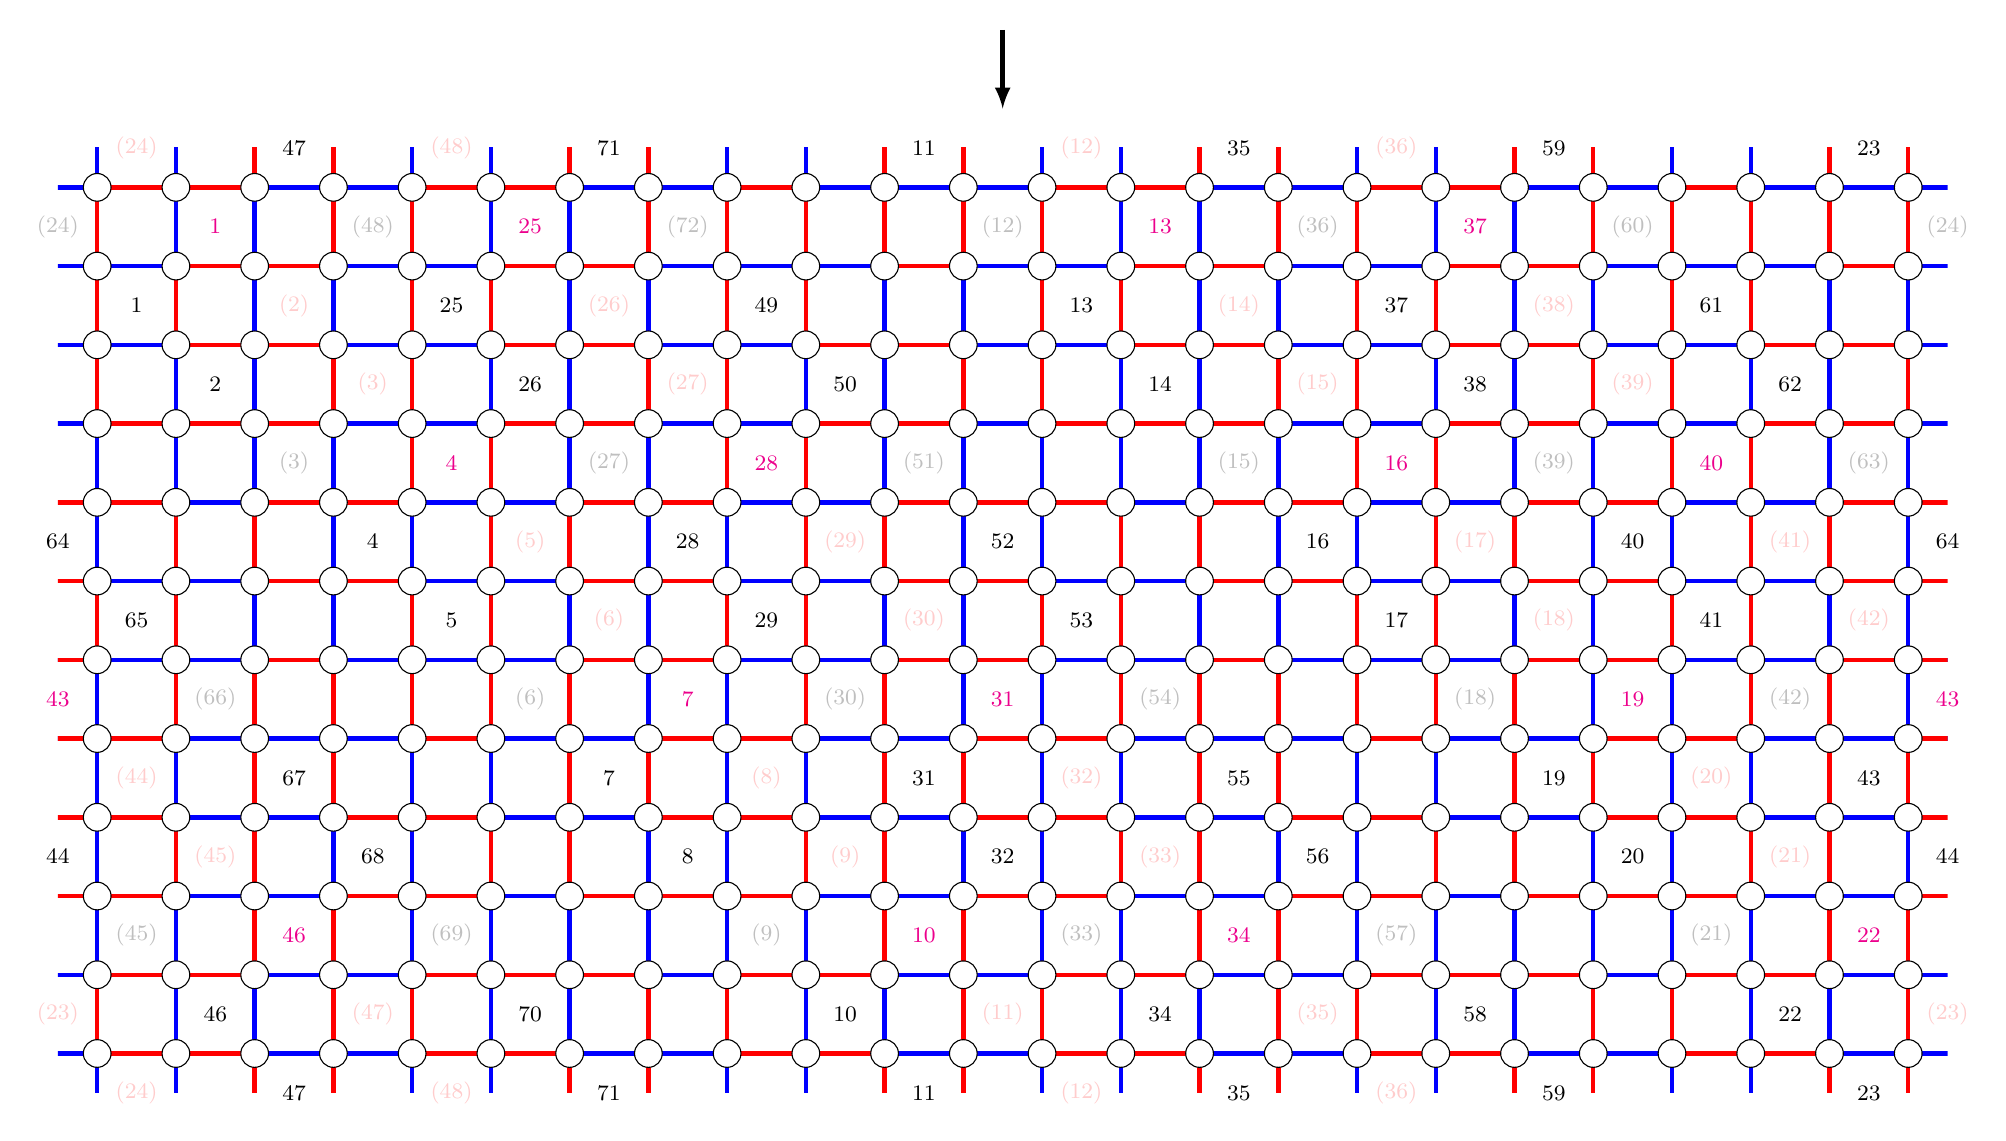
\begin{tikzpicture}
            \draw [-latex, ultra thick] (11.5,13) -- (11.5,12);
            
            \foreach \i in {1,2,...,11}{
                \node [align=center] at (\i-0.5, 10.5-\i) {\ifthenelse{\i=3 \OR \i=6 \OR \i=9}{\textcolor{gray!50}{\footnotesize $(\i)$}}{\footnotesize $\i$}};
            }
            \foreach \i in {11,12,...,23}{
                \node [align=center] at (\i-0.5, 10.5-\i+12) {\ifthenelse{\i=12 \OR \i=15 \OR \i=18 \OR \i=21}{\textcolor{gray!50}{\footnotesize $(\i)$}}{\footnotesize $\i$}};
            }
            \foreach \i in {23,24}{
                \node [align=center] at (\i-0.5, 10.5-\i+24) {\ifthenelse{\i=24}{\textcolor{gray!50}{\footnotesize $(\i)$}}{\footnotesize $\i$}};
            }
            \node [align=center] at (-0.5, 10.5) {\textcolor{gray!50}{\footnotesize $(24)$}};
            \foreach \i in {25,26,...,35}{
                \node [align=center] at (\i-0.5-20, 10.5-\i+24) {\ifthenelse{\i=27 \OR \i=30 \OR \i=33}{\textcolor{gray!50}{\footnotesize $(\i)$}}{\footnotesize $\i$}};
            }
            \foreach \i in {35,36,...,44}{
                \node [align=center] at (\i-0.5-20, 10.5-\i+36) {\ifthenelse{\i=36 \OR \i=39 \OR \i=42}{\textcolor{gray!50}{\footnotesize $(\i)$}}{\footnotesize $\i$}};
            }
            \foreach \i in {44,45,...,47}{
                \node [align=center] at (\i-0.5-44, 10.5-\i+36) {\ifthenelse{\i=45}{\textcolor{gray!50}{\footnotesize $(\i)$}}{\footnotesize $\i$}};
            }
            \node [align=center] at (2.5, 11.5) {\footnotesize $47$};
            \node [align=center] at (3.5, 10.5) {\textcolor{gray!50}{\footnotesize $(48)$}};
            
            \foreach \i in {49,50,...,59}{
                \node [align=center] at (\i-0.5-40, 10.5-\i+48) {\ifthenelse{\i=51 \OR \i=54 \OR \i=57}{\textcolor{gray!50}{\footnotesize $(\i)$}}{\footnotesize $\i$}};
            }
            \foreach \i in {59, 60,...,64}{
                \node [align=center] at (\i-0.5-40, 10.5-\i+60) {\ifthenelse{\i=60 \OR \i=63}{\textcolor{gray!50}{\footnotesize $(\i)$}}{\footnotesize $\i$}};
            }
            \foreach \i in {64,65,...,71}{
                \node [align=center] at (\i-0.5-64, 10.5-\i+60) {\ifthenelse{\i=66 \OR \i=69}{\textcolor{gray!50}{\footnotesize $(\i)$}}{\footnotesize $\i$}};
            }
            \node [align=center] at (6.5, 11.5) {\footnotesize $71$};
            \node [align=center] at (7.5, 10.5) {\textcolor{gray!50}{\footnotesize $(72)$}};
            
            % T's
            \foreach \i in {1,2,...,12}{
                \node [align=center] at (\i+0.5, 11.5-\i) {\ifthenelse{\i=1 \OR \i=4 \OR \i=7 \OR \i=10}{\textcolor{magenta}{\footnotesize $\i$}}{\textcolor{pink!80}{\footnotesize $(\i)$}}};
            }
            \foreach \i in {12,13,...,23}{
                \node [align=center] at (\i+0.5, 11.5-\i+12) {\ifthenelse{\i=13 \OR \i=16 \OR \i=19 \OR \i=22}{\textcolor{magenta}{\footnotesize $\i$}}{\textcolor{pink!80}{\footnotesize $(\i)$}}};
            }
            \node [align=center] at (0.5, -0.5) {\textcolor{pink!80}{\footnotesize $(24)$}};
            \node [align=center] at (-0.5, 0.5) {\textcolor{pink!80}{\footnotesize $(23)$}};
            \node [align=center] at (0.5, 11.5) {\textcolor{pink!80}{\footnotesize $(24)$}};
            \foreach \i in {25,26,...,36}{
                \node [align=center] at (\i+0.5-20, 11.5-\i+24) {\ifthenelse{\i=25 \OR \i=28 \OR \i=31 \OR \i=34}{\textcolor{magenta}{\footnotesize $\i$}}{\textcolor{pink!80}{\footnotesize $(\i)$}}};
            }
            \foreach \i in {36,37,...,43}{
                \node [align=center] at (\i+0.5-20, 11.5-\i+36) {\ifthenelse{\i=37 \OR \i=40 \OR \i=43 \OR \i=34}{\textcolor{magenta}{\footnotesize $\i$}}{\textcolor{pink!80}{\footnotesize $(\i)$}}};
            }
            \foreach \i in {43,44,...,48}{
                \node [align=center] at (\i+0.5-44, 11.5-\i+36) {\ifthenelse{\i=43 \OR \i=46}{\textcolor{magenta}{\footnotesize $\i$}}{\textcolor{pink!80}{\footnotesize $(\i)$}}};
            }
            \node [align=center] at (4.5, 11.5) {\textcolor{pink!80}{\footnotesize $(48)$}};
            
            \clip (-0.5, -0.5) rectangle (23.5, 11.5);
            \foreach \i in {0,4,...,24}{
                \draw [ultra thick, -, color=blue] (\i-1,8) -- (\i, 8) -- (\i, 6) -- (\i+2, 6) -- (\i+2, 5) -- (\i-1, 5) -- (\i-1, 8);
                \draw [ultra thick, -, color=red] (\i, 8) -- (\i, 11) -- (\i+1, 11) -- (\i+1, 9) -- (\i+3, 9) -- (\i+3,8) -- (\i, 8);
            }
            \foreach \i in {-2,2,...,26}{
                \draw [ultra thick, -, color=red] (\i, 2) -- (\i, 5) -- (\i+1, 5) -- (\i+1, 3) -- (\i+3, 3) -- (\i+3,2) -- (\i, 2);
                \draw [ultra thick, -, color=blue] (\i-1,4) -- (\i+2, 4) -- (\i+2,1) -- (\i+1,1) -- (\i+1, 3) -- (\i-1,3) -- (\i-1,4);
                \draw [ultra thick, -, color=red] (\i, 7) -- (\i+3, 7) -- (\i+3, 4) -- (\i+2, 4) -- (\i+2,6) -- (\i,6) -- (\i, 7);
                \draw [ultra thick, -, color=blue] (\i-3,10) -- (\i,10) -- (\i,7) -- (\i-1,7) -- (\i-1,9) -- (\i-3,9) -- (\i-3,10);
                \draw [ultra thick, -, color=blue] (\i-1,2) -- (\i,2) -- (\i,0) -- (\i+2,0) -- (\i+2,-1) -- (\i-1,-1) -- (\i-1,2);
                 \draw [ultra thick, -, color=blue] (\i-1,14) -- (\i,14) -- (\i,12) -- (\i+2,12) -- (\i+2,11) -- (\i-1,11) -- (\i-1,14);
            }
            \foreach \i in {0,4,...,24}{
                \draw [ultra thick, -, color=red] (\i, 13) -- (\i+3, 13) -- (\i+3, 10) -- (\i+2, 10) -- (\i+2,12) -- (\i,12) -- (\i, 13);
                \draw [ultra thick, -, color=red] (\i, 1) -- (\i+3, 1) -- (\i+3, -1) -- (\i+2, -1) -- (\i+2,0) -- (\i,0) -- (\i, 1);
            }
            
            \foreach \i in {1,5,13,17}{
                \draw [ultra thick, -, color=red] (\i,10) -- (\i+1, 10);
                \draw [ultra thick, -, color=red] (\i,11) -- (\i+1, 11);
                \draw [ultra thick, -, color=blue] (\i, 10) -- (\i, 11);
                \draw [ultra thick, -, color=blue] (\i+1, 10) -- (\i+1, 11);
            }
            
            \foreach \i in {4,8,16,20}{
                \draw [ultra thick, -, color=blue] (\i,7) -- (\i+1, 7);
                \draw [ultra thick, -, color=blue] (\i,8) -- (\i+1, 8);
                \draw [ultra thick, -, color=red] (\i, 7) -- (\i, 8);
                \draw [ultra thick, -, color=red] (\i+1, 7) -- (\i+1, 8);
            }
            \foreach \i in {-1,7,11,19,23}{
                \draw [ultra thick, -, color=red] (\i,4) -- (\i+1, 4);
                \draw [ultra thick, -, color=red] (\i,5) -- (\i+1, 5);
                \draw [ultra thick, -, color=blue] (\i, 4) -- (\i, 5);
                \draw [ultra thick, -, color=blue] (\i+1, 4) -- (\i+1, 5);
            }
            \foreach \i in {2,10,14,22}{
                \draw [ultra thick, -, color=blue] (\i,1) -- (\i+1, 1);
                \draw [ultra thick, -, color=blue] (\i,2) -- (\i+1, 2);
                \draw [ultra thick, -, color=red] (\i, 1) -- (\i, 2);
                \draw [ultra thick, -, color=red] (\i+1, 1) -- (\i+1, 2);
            }
        
            \foreach \i in {0,1,...,23}{\foreach \j in {0,1,...,11}{\filldraw[fill=white, draw=black] (\i, \j) circle (5pt);}}
        \end{tikzpicture}
    \end{center}
    
    This method produces most of the possible decompositions of $C_m \sq C_n$ when $m$ and $n$ are multiples of $4$.
    
    }
    
    \column{0.25}
    \block{Decomposing into 3 Cycles}{
        \begin{theorem}
            If $3 \mid m$ or $3 \mid n$, then it is possible to decompose $C_m \sq C_n$ into three cycles of length $\frac{2mn}{3}$.
        \end{theorem}
\textbf{Proof:}
Without loss of generality, assume $3 \mid n$.\\
If $m$ is odd, \hspace{6.5cm} \emph{Structure for arbitrary size:}
\begin{center}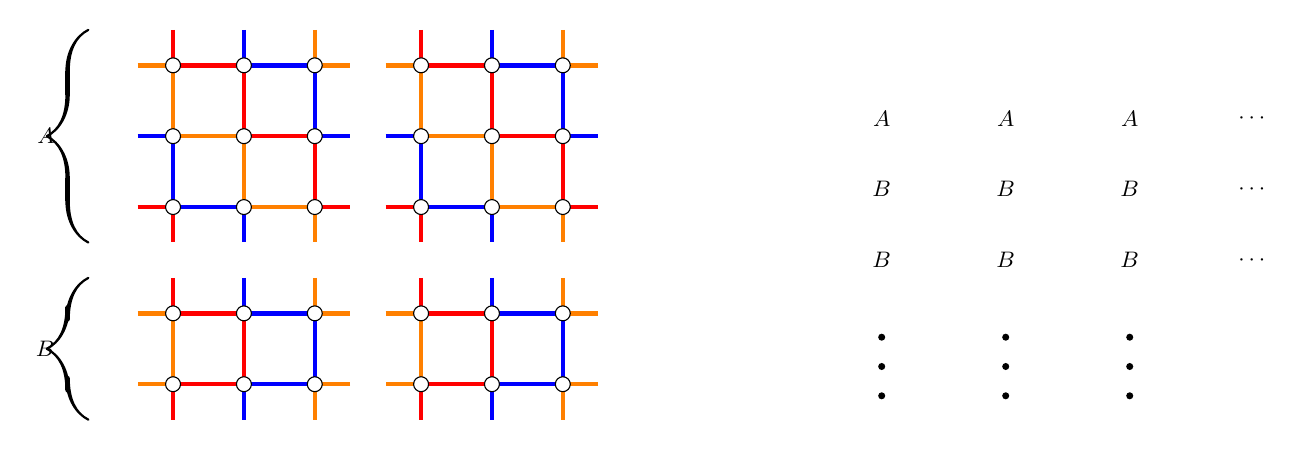
\begin{tikzpicture}[scale=.9, transform shape]
% First A block
    \draw[red, ultra thick] (-.5, -2) -- (0, -2) -- (0, -2.5); \draw[blue, ultra thick] (-.5, -1) -- (0, -1) -- (0, -2) -- (1, -2) -- (1, -2.5); \draw[orange, ultra thick] (-.5, 0) -- (0, 0) -- (0, -1) -- (1, -1) -- (1, -2) -- (2, -2) -- (2, -2.5); \draw[red, ultra thick] (0, .5) -- (0, 0) -- (1, 0) -- (1, -1) -- (2, -1) -- (2, -2) -- (2.5, -2); \draw[blue, ultra thick] (1, .5) -- (1, 0) -- (2, 0) -- (2, -1) -- (2.5, -1); \draw[orange, ultra thick] (2, .5) -- (2, 0) -- (2.5, 0); \foreach \x in {0, 1, 2}{\foreach \y in {0, -1, -2}{\draw[draw = black, fill = white] (\x, \y) circle (3pt);}}\draw [ultra thick, decorate, decoration = {calligraphic brace, raise=5pt, amplitude=15pt}] (-1, -2.5) --  (-1, .5) node[pos=.5, left=15pt, black]{\small{$A$}};
% Second A block
    \draw[red, ultra thick] (3, -2) -- (3.5, -2) -- (3.5, -2.5); \draw[blue, ultra thick] (3, -1) -- (3.5, -1) -- (3.5, -2) -- (4.5, -2) -- (4.5, -2.5); \draw[orange, ultra thick] (3, 0) -- (3.5, 0) -- (3.5, -1) -- (4.5, -1) -- (4.5, -2) -- (5.5, -2) -- (5.5, -2.5); \draw[red, ultra thick] (3.5, .5) -- (3.5, 0) -- (4.5, 0) -- (4.5, -1) -- (5.5, -1) -- (5.5, -2) -- (6, -2); \draw[blue, ultra thick] (4.5, .5) -- (4.5, 0) -- (5.5, 0) -- (5.5, -1) -- (6, -1); \draw[orange, ultra thick] (5.5, .5) -- (5.5, 0) -- (6, 0); \foreach \x in {3.5, 4.5, 5.5}{\foreach \y in {0, -1, -2}{\draw[draw = black, fill = white] (\x, \y) circle (3pt);}}
% First B block
    \draw[red, ultra thick] (0, -3) -- (0, -3.5) -- (1, -3.5) -- (1, -4.5) -- (0, -4.5) -- (0, -5); \draw[blue, ultra thick] (1, -3) -- (1, -3.5) -- (2, -3.5) -- (2, -4.5) -- (1, -4.5) -- (1, -5); \draw[orange, ultra thick] (-.5, -3.5) -- (0, -3.5) -- (0, -4.5) -- (-.5, -4.5); \draw[orange, ultra thick] (2, -3) -- (2, -3.5) -- (2.5, -3.5); \draw[orange, ultra thick] (2.5, -4.5) -- (2, -4.5) -- (2, -5); \foreach \x in {0, 1, 2}{\foreach \y in {-3.5, -4.5}{\draw[draw = black, fill = white] (\x, \y) circle (3pt);}}\draw [ultra thick, decorate, decoration = {calligraphic brace, raise=5pt, amplitude=15pt}] (-1, -5) --  (-1, -3) node[pos=.5, left=15pt, black]{\small{$B$}};
% Second B block
   \draw[red, ultra thick] (3.5, -3) -- (3.5, -3.5) -- (4.5, -3.5) -- (4.5, -4.5) -- (3.5, -4.5) -- (3.5, -5); \draw[blue, ultra thick] (4.5, -3) -- (4.5, -3.5) -- (5.5, -3.5) -- (5.5, -4.5) -- (4.5, -4.5) -- (4.5, -5); \draw[orange, ultra thick] (3, -3.5) -- (3.5, -3.5) -- (3.5, -4.5) -- (3, -4.5); \draw[orange, ultra thick] (5.5, -3) -- (5.5, -3.5) -- (6, -3.5); \draw[orange, ultra thick] (6, -4.5) -- (5.5, -4.5) -- (5.5, -5); \foreach \x in {3.5, 4.5, 5.5}{\foreach \y in {-3.5, -4.5}{\draw[draw = black, fill = white] (\x, \y) circle (3pt);}}
%A/B Table
   \small{\node at (10, -.75){$A$}; \node at (10, -1.75){$B$}; \node at (10, -2.75){$B$}; \vvdots{10}{-4.25}; \node at (11.75, -.75){$A$}; \node at (11.75, -1.75){$B$}; \node at (11.75, -2.75){$B$}; \vvdots{11.75}{-4.25};\node at (13.5, -.75){$A$}; \node at (13.5, -1.75){$B$}; \node at (13.5, -2.75){$B$}; \vvdots{13.5}{-4.25};} \node at (15.25, -.75){$\cdots$}; \node at (15.25, -1.75){$\cdots$}; \node at (15.25, -2.75){$\cdots$};
\end{tikzpicture}\end{center}
If $m$ is even,\\
\textbf{Case 1:} $n = 3$
\begin{center}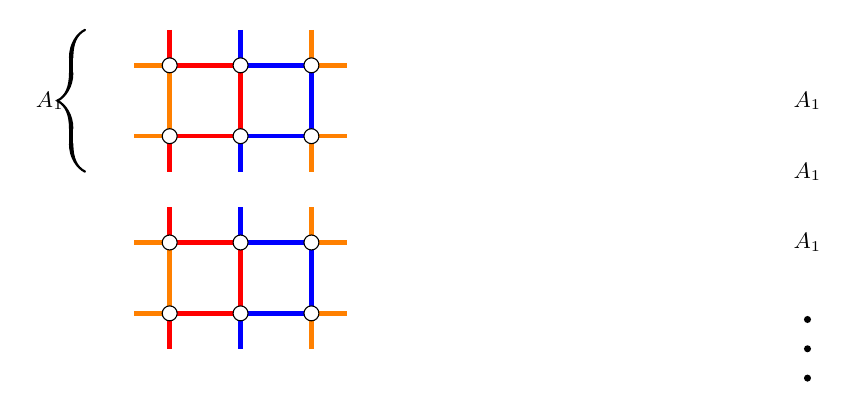
\begin{tikzpicture}[scale=.9, transform shape]
% First Block
    \draw[red, ultra thick] (0, -3) -- (0, -3.5) -- (1, -3.5) -- (1, -4.5) -- (0, -4.5) -- (0, -5); \draw[blue, ultra thick] (1, -3) -- (1, -3.5) -- (2, -3.5) -- (2, -4.5) -- (1, -4.5) -- (1, -5); \draw[orange, ultra thick] (-.5, -3.5) -- (0, -3.5) -- (0, -4.5) -- (-.5, -4.5); \draw[orange, ultra thick] (2, -3) -- (2, -3.5) -- (2.5, -3.5); \draw[orange, ultra thick] (2.5, -4.5) -- (2, -4.5) -- (2, -5); \foreach \x in {0, 1, 2}{\foreach \y in {-3.5, -4.5}{\draw[draw = black, fill = white] (\x, \y) circle (3pt);}}\draw [ultra thick, decorate, decoration = {calligraphic brace, raise=5pt, amplitude=10pt}] (-1, -5) --  (-1, -3) node[pos=.5, left=10pt, black]{\small{$A_1$}};
%Second Block
    \draw[red, ultra thick] (0, -5.5) -- (0, -6) -- (1, -6) -- (1, -7) -- (0, -7) -- (0, -7.5); \draw[blue, ultra thick] (1, -5.5) -- (1, -6) -- (2, -6) -- (2, -7) -- (1, -7) -- (1, -7.5); \draw[orange, ultra thick] (-.5, -6) -- (0, -6) -- (0, -7) -- (-.5, -7); \draw[orange, ultra thick] (2, -5.5) -- (2, -6) -- (2.5, -6); \draw[orange, ultra thick] (2.5, -7) -- (2, -7) -- (2, -7.5); \foreach \x in {0, 1, 2}{\foreach \y in {-6, -7}{\draw[draw = black, fill = white] (\x, \y) circle (3pt);}}
%Table
    \small{ \node at (9, -4){$A_1$}; \node at (9, -5){$A_1$}; \node at (9, -6){$A_1$};\vvdots{9}{-7.5};} 
\end{tikzpicture}\end{center}
\textbf{Case 2:} $m = 4$\\
2a) $n$ is even
\begin{center}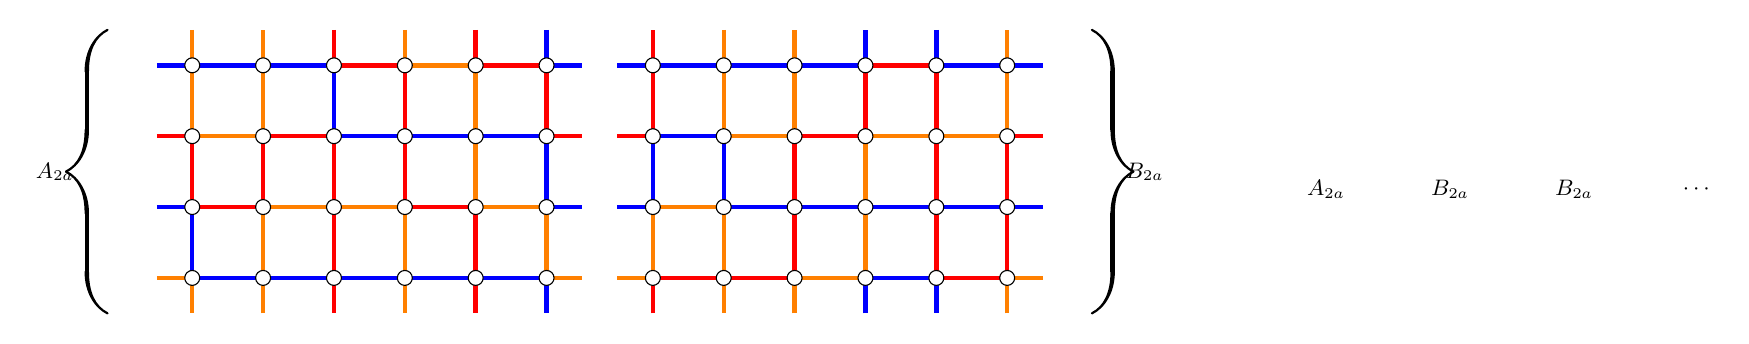
\begin{tikzpicture}[scale=.9, transform shape]
%A Block
    \draw[blue, ultra thick] (-.5, 0) -- (2, 0) -- (2, -1) -- (5, -1) -- (5, -2) -- (5.5, -2); \draw[blue, ultra thick] (-.5, -2) -- (0, -2) -- (0, -3) -- (5, -3) -- (5, -3.5); \draw[blue, ultra thick] (5, .5) -- (5, 0) -- (5.5, 0);
    \draw[orange, ultra thick] (0, .5) -- (0, -1) -- (1, -1) -- (1, .5); \draw[orange, ultra thick] (3, .5) -- (3, 0) -- (4, 0) -- (4, -2) -- (5, -2) -- (5, -3) -- (5.5, -3); \draw[orange, ultra thick] (-.5, -3) -- (0, -3) -- (0, -3.5); \draw[orange, ultra thick] (1, -3.5) -- (1, -2) -- (3, -2) -- (3, -3.5);
    \draw[red, ultra thick] (-.5, -1) -- (0, -1) -- (0, -2) -- (1, -2) -- (1, -1) -- (2, -1) -- (2, -3.5); \draw[red, ultra thick] (2, .5) -- (2, 0) -- (3, 0) -- (3, -2) -- (4, -2) -- (4, -3.5); \draw[red, ultra thick] (4, .5) -- (4, 0) -- (5, 0) -- (5, -1) -- (5.5, -1);
    \foreach \x in {0, 1, ..., 5}{\foreach \y in {0, -1, -2, -3}{\filldraw[draw=black, fill=white] (\x, \y) circle (3pt);}}\draw [ultra thick, decorate, decoration = {calligraphic brace, raise=5pt, amplitude=15pt}] (-1, -3.5) --  (-1, .5) node[pos=.5, left=15pt, black]{\small{$A_{2a}$}};
%B Block
    \draw[blue, ultra thick] (6, 0) -- (9.5, 0) -- (9.5, .5); \draw[blue, ultra thick] (10.5, .5) -- (10.5, 0) -- (12, 0); \draw[blue, ultra thick] (6, -2) -- (6.5, -2) -- (6.5, -1) -- (7.5, -1) -- (7.5, -2) -- (12, -2); \draw[blue, ultra thick] (9.5, -3.5) -- (9.5, -3) -- (10.5, -3) -- (10.5, -3.5);
    \draw[orange, ultra thick] (7.5, .5) -- (7.5, -1) -- (8.5, -1) -- (8.5, .5); \draw[orange, ultra thick] (6, -3) -- (6.5, -3) -- (6.5, -2) -- (7.5, -2) -- (7.5, -3.5); \draw[orange, ultra thick] (8.5, -3.5) -- (8.5, -3) -- (9.5, -3) -- (9.5, -1) -- (11.5, -1) -- (11.5, .5); \draw[orange, ultra thick] (11.5, -3.5) -- (11.5, -3) -- (12, -3);
    \draw[red, ultra thick] (6, -1) -- (6.5, -1) -- (6.5, .5); \draw[red, ultra thick] (6.5, -3.5) -- (6.5, -3) -- (8.5, -3) -- (8.5, -1) -- (9.5, -1) -- (9.5, 0) -- (10.5, 0) -- (10.5, -3) -- (11.5, -3) -- (11.5, -1) -- (12, -1);
    \foreach \x in {6.5, 7.5, 8.5, 9.5, 10.5, 11.5}{\foreach \y in {0, -1, -2, -3}{\filldraw[draw=black, fill=white] (\x, \y) circle (3pt);}}\draw [ultra thick, decorate, decoration = {calligraphic brace, raise=5pt, amplitude=15pt}] (12.5, .5) --  (12.5, -3.5) node[pos=.5, right=15pt, black]{\small{$B_{2a}$}};
%Table
    \small{\node at (16, -1.75){$A_{2a}$}; \node at (17.75, -1.75){$B_{2a}$}; \node at (19.5, -1.75){$B_{2a}$};} \node at (21.25, -1.75){$\cdots$};
\end{tikzpicture}\end{center}
2b) $n$ is odd
\begin{center}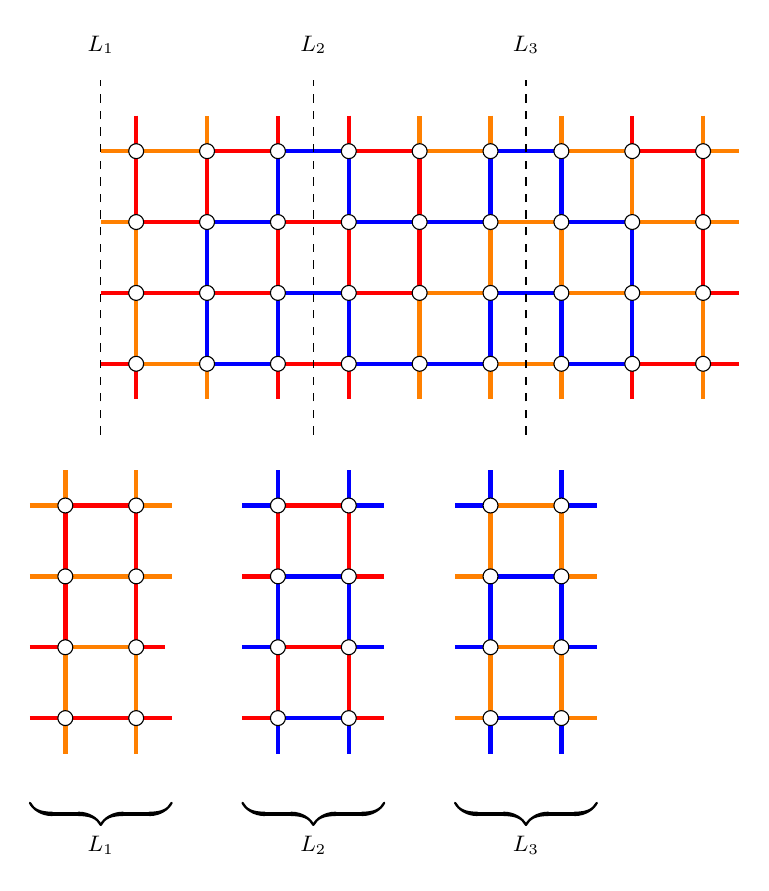
\begin{tikzpicture}[scale=.9, transform shape]
%Main Block
    \draw[red, ultra thick] (0,3.5) -- (0,2) -- (1,2) -- (1,3) -- (2,3) -- (2,3.5);
    \draw[red, ultra thick] (2,-0.5) -- (2,0) -- (3,0) -- (3,-0.5);
    \draw[red, ultra thick] (3,3.5) -- (3,3) -- (4,3) -- (4,1) -- (3,1) -- (3,2) -- (2,2) -- (2,1) -- (-0.5,1);
    \draw[red, ultra thick] (8.5,1) -- (8,1) -- (8,3) -- (7,3) -- (7,3.5);
    \draw[red, ultra thick] (7, -0.5) -- (7,0) -- (8.5,0);
    \draw[red, ultra thick] (-0.5,0) -- (0,0) -- (0,-0.5);
    \draw[blue, ultra thick] (1,2) -- (1,0) -- (2,0) -- (2,1) -- (3,1) -- (3,0) -- (5,0) -- (5,1) -- (6,1) -- (6,0) -- (7,0) -- (7,2) -- (6,2) -- (6,3) -- (5,3) -- (5,2) -- (3,2) -- (3,3) -- (2,3) -- (2,2) -- (1,2);
    \draw[orange, ultra thick] (-0.5,3) -- (1,3) -- (1,3.5);
    \draw[orange, ultra thick] (1,-0.5) -- (1,0) -- (0,0) -- (0,2) -- (-0.5,2);
    \draw[orange, ultra thick] (8.5,2) -- (7,2) -- (7,3) -- (6,3) -- (6,3.5);
    \draw[orange, ultra thick] (6,-0.5) -- (6,0) -- (5,0) -- (5,-0.5);
    \draw[orange, ultra thick] (5,3.5) -- (5,3) -- (4,3) -- (4,3.5);
    \draw[orange, ultra thick] (4,-0.5) -- (4,1) -- (5,1) -- (5,2) -- (6,2) -- (6,1) -- (8,1) -- (8,-0.5);
    \draw[orange, ultra thick] (8, 3.5) -- (8,3) -- (8.5,3);
    \foreach \i in {0,1,...,8}{\foreach \j in {0,1,...,3}{\filldraw[fill=white, draw=black] (\i, \j) circle (3pt);}}
%Lines
    \draw[dashed] (-.5, -1) -- (-.5, 4); \node at (-.5, 4.5) {\small{$L_1$}}; \draw[dashed] (2.5, -1) -- (2.5, 4);\node at (2.5, 4.5) {\small{$L_2$}}; \draw[dashed] (5.5, -1) -- (5.5, 4); \node at (5.5, 4.5) {\small{$L_3$}};
%L1 block
    \draw[red, ultra thick] (-1.5, -4) -- (-1, -4) -- (-1, -2) -- (0, -2) -- (0, -4) -- (.4, -4); \draw[red, ultra thick] (-1.5, -5) -- (.5, -5);
    \draw[orange, ultra thick] (-1.5, -2) -- (-1, -2) -- (-1, -1.5); \draw[orange, ultra thick] (.5, -2) -- (0, -2) -- (0, -1.5); \draw[orange, ultra thick] (-1.5, -3) -- (.5, -3); \draw[orange, ultra thick] (-1, -5.5) -- (-1, -4) -- (0, -4) -- (0, -5.5); \foreach \i in {-1, 0}{\foreach \j in {-2, -3, ..., -5}{\filldraw[fill=white, draw=black] (\i, \j) circle (3pt);}}\draw [ultra thick, decorate, decoration = {calligraphic brace, raise=5pt, amplitude=8pt}] (.5, -6) --  (-1.5, -6) node[pos=.5, below=15pt, black]{\small{$L_1$}};
%L2 block
    \draw[blue, ultra thick] (1.5, -2) -- (2, -2) -- (2, -1.5); \draw[blue, ultra thick] (3, -1.5) -- (3, -2) -- (3.5, -2); \draw[blue, ultra thick] (1.5, -4) -- (2, -4) -- (2, -3) -- (3, -3) -- (3, -4) -- (3.5, -4); \draw[blue, ultra thick] (2, -5.5) -- (2, -5) -- (3, -5) -- (3, -5.5); \draw[red, ultra thick] (1.5, -5) -- (2, -5) -- (2, -4) -- (3, -4) -- (3, -5) -- (3.5, -5);\draw[red, ultra thick] (1.5, -3) -- (2, -3) -- (2, -2) -- (3, -2) -- (3, -3) -- (3.5, -3);\foreach \i in {2, 3}{\foreach \j in {-2, -3,..., -5}{\filldraw[fill=white, draw=black] (\i, \j) circle (3pt);}}\draw [ultra thick, decorate, decoration = {calligraphic brace, raise=5pt, amplitude=8pt}] (3.5, -6) --  (1.5, -6) node[pos=.5, below=15pt, black]{\small{$L_2$}};
%L3 block
    \draw[blue, ultra thick] (4.5, -2) -- (5, -2) -- (5, -1.5); \draw[blue, ultra thick] (6, -1.5) -- (6, -2) -- (6.5, -2); \draw[blue, ultra thick] (4.5, -4) -- (5, -4) -- (5, -3) -- (6, -3) -- (6, -4) -- (6.5, -4); \draw[blue, ultra thick] (5, -5.5) -- (5, -5) -- (6, -5) -- (6, -5.5); \draw[orange, ultra thick] (4.5, -5) -- (5, -5) -- (5, -4) -- (6, -4) -- (6, -5) -- (6.5, -5);\draw[orange, ultra thick] (4.5, -3) -- (5, -3) -- (5, -2) -- (6, -2) -- (6, -3) -- (6.5, -3);\foreach \i in {5, 6}{\foreach \j in {-2, -3,..., -5}{\filldraw[fill=white, draw=black] (\i, \j) circle (3pt);}}\draw [ultra thick, decorate, decoration = {calligraphic brace, raise=5pt, amplitude=8pt}] (6.5, -6) --  (4.5, -6) node[pos=.5, below=15pt, black]{\small{$L_3$}};
\end{tikzpicture}\end{center}
\textbf{Case 3:} $m \geq 6$\\
3a) $n$ is even
\begin{center}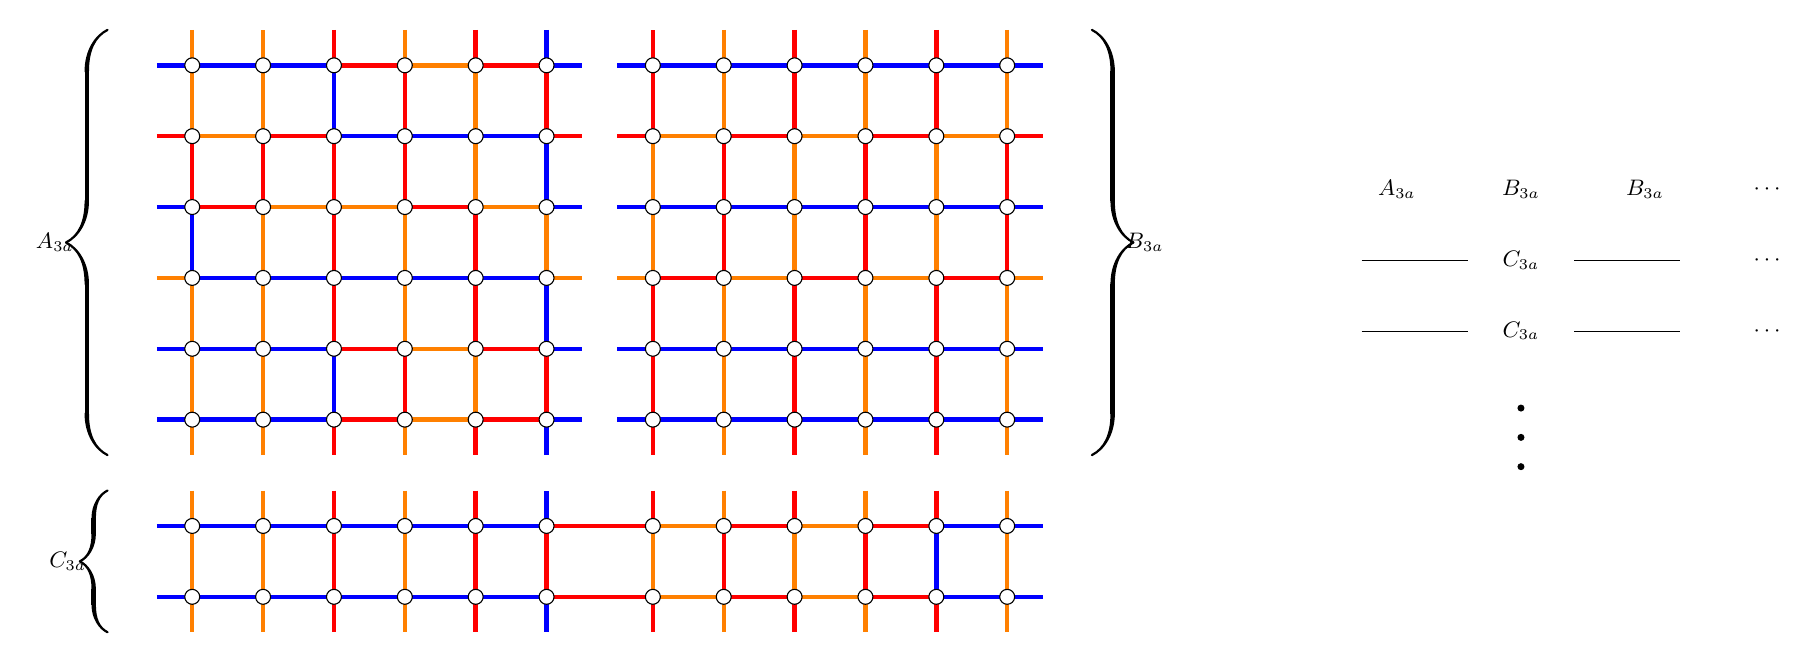
\begin{tikzpicture}[scale=.9, transform shape]
%A Block
    \draw[blue, ultra thick] (-.5, 0) -- (2, 0) -- (2, -1) -- (5, -1) -- (5, -2) -- (5.5, -2); \draw[blue, ultra thick] (-.5, -2) -- (0, -2) -- (0, -3) -- (5, -3) -- (5, -4) -- (5.5, -4); \draw[blue, ultra thick] (5, .5) -- (5, 0) -- (5.5, 0); \draw[blue, ultra thick] (5.5, -5) -- (5, -5) -- (5, -5.5); \draw[blue, ultra thick] (-.5, -4) -- (2, -4) -- (2, -5) -- (-.5, -5);
    \draw[orange, ultra thick] (0, .5) -- (0, -1) -- (1, -1) -- (1, .5); \draw[orange, ultra thick] (3, .5) -- (3, 0) -- (4, 0) -- (4, -2) -- (5, -2) -- (5, -3) -- (5.5, -3); \draw[orange, ultra thick] (-.5, -3) -- (0, -3) -- (0, -5.5); \draw[orange, ultra thick] (1, -5.5)  -- (1, -2) -- (3, -2) -- (3, -4) -- (4, -4) -- (4, -5) -- (3, -5) -- (3, -5.5);
    \draw[red, ultra thick] (-.5, -1) -- (0, -1) -- (0, -2) -- (1, -2) -- (1, -1) -- (2, -1) -- (2, -4) -- (3, -4) -- (3, -5) -- (2, -5) -- (2, -5.5); \draw[red, ultra thick] (2, .5) -- (2, 0) -- (3, 0) -- (3, -2) -- (4, -2) -- (4, -4) -- (5, -4) -- (5, -5) -- (4, -5) -- (4, -5.5); \draw[red, ultra thick] (4, .5) -- (4, 0) -- (5, 0) -- (5, -1) -- (5.5, -1);
    \foreach \x in {0, 1, ..., 5}{\foreach \y in {0, -1, ..., -5}{\filldraw[draw=black, fill=white] (\x, \y) circle (3pt);}}\draw [ultra thick, decorate, decoration = {calligraphic brace, raise=5pt, amplitude=15pt}] (-1, -5.5) --  (-1, .5) node[pos=.5, left=15pt, black]{\small{$A_{3a}$}};
%B Block
    \draw[blue, ultra thick] (6, 0) -- (12, 0); \draw[blue, ultra thick] (6, -2) -- (12, -2); \draw[blue, ultra thick] (6, -4) -- (12, -4); \draw[blue, ultra thick] (6, -5) -- (12, -5);
    \draw[red, ultra thick] (6, -1) -- (6.5, -1) -- (6.5, .5); \draw[red, ultra thick] (8.5, .5) -- (8.5, -1) -- (7.5, -1) -- (7.5, -3) -- (6.5, -3) -- (6.5, -5.5); \draw[red, ultra thick] (10.5, .5) -- (10.5, -1) -- (9.5, -1) -- (9.5, -3) -- (8.5, -3) -- (8.5, -5.5); \draw[red, ultra thick] (12, -1) -- (11.5, -1) -- (11.5, -3) -- (10.5, -3) -- (10.5, -5.5);
    \draw[orange, ultra thick] (7.5, .5) -- (7.5, -1) -- (6.5, -1) -- (6.5, -3) -- (6, -3); \draw[orange, ultra thick] (9.5, .5) -- (9.5, -1) -- (8.5, -1) -- (8.5, -3) -- (7.5, -3) -- (7.5, -5.5); \draw[orange, ultra thick] (11.5, .5) -- (11.5, -1) -- (10.5, -1) -- (10.5, -3) -- (9.5, -3) -- (9.5, -5.5); \draw[orange, ultra thick] (12, -3) -- (11.5, -3) -- (11.5, -5.5);
    \foreach \x in {6.5, 7.5, 8.5, 9.5, 10.5, 11.5}{\foreach \y in {0, -1, ..., -5}{\filldraw[draw=black, fill=white] (\x, \y) circle (3pt);}}\draw [ultra thick, decorate, decoration = {calligraphic brace, raise=5pt, amplitude=15pt}] (12.5, .5) --  (12.5, -5.5) node[pos=.5, right=15pt, black]{\small{$B_{3a}$}};
%C Block
    \draw[blue, ultra thick] (-.5, -6.5) -- (5, -6.5) -- (5, -6); \draw[blue, ultra thick] (-.5, -7.5) -- (5, -7.5) -- (5, -8); \draw[blue, ultra thick] (12, -6.5) -- (10.5, -6.5) -- (10.5, -7.5) -- (12, -7.5); 
    \draw[orange, ultra thick] (0, -6) -- (0, -8); \draw[orange, ultra thick] (1, -6) -- (1, -8); \draw[orange, ultra thick] (3, -6) -- (3, -8); 
    \draw[orange, ultra thick] (7.5, -6) -- (7.5, -6.5) -- (6.5, -6.5) -- (6.5, -7.5) -- (7.5, -7.5) -- (7.5, -8); \draw[orange, ultra thick] (9.5, -6) -- (9.5, -6.5) -- (8.5, -6.5) -- (8.5, -7.5) -- (9.5, -7.5) -- (9.5, -8); \draw[orange, ultra thick] (11.5, -6) -- (11.5, -8);
    \draw[red, ultra thick] (2, -6) -- (2, -8);\draw[red, ultra thick] (4, -6) -- (4, -8); \draw[red, ultra thick] (6.5, -6) -- (6.5, -6.5) -- (5, -6.5) -- (5, -7.5) -- (6.5, -7.5) -- (6.5, -8); \draw[red, ultra thick] (8.5, -6) -- (8.5, -6.5) -- (7.5, -6.5) -- (7.5, -7.5) -- (8.5, -7.5) -- (8.5, -8);\draw[red, ultra thick] (10.5, -6) -- (10.5, -6.5) -- (9.5, -6.5) -- (9.5, -7.5) -- (10.5, -7.5) -- (10.5, -8);
    \foreach \x in {0, 1, 2, 3, 4, 5, 6.5, 7.5, 8.5, 9.5, 10.5, 11.5}{\foreach \y in {-6.5, -7.5}{\filldraw[draw=black, fill=white] (\x, \y) circle (3pt);}}\draw [ultra thick, decorate, decoration = {calligraphic brace, raise=5pt, amplitude=10pt}] (-1, -8) --  (-1, -6) node[pos=.5, left=10pt, black]{\small{$C_{3a}$}};
%Table
    \small{\node at (17, -1.75){$A_{3a}$}; \draw (16.5, -2.75) -- (18, -2.75); \draw (19.5, -2.75) -- (21, -2.75); \node at (18.75, -1.75){$B_{3a}$}; \node at (18.75, -2.75){$C_{3a}$}; \vvdots{18.75}{-5.25}; \node at (18.75, -3.75){$C_{3a}$}; \node at (20.5, -1.75){$B_{3a}$};\draw (16.5, -3.75) -- (18, -3.75); \draw (19.5, -3.75) -- (21, -3.75);} \node at (22.25, -1.75){$\cdots$}; \node at (22.25, -2.75){$\cdots$}; \node at (22.25, -3.75){$\cdots$};
\end{tikzpicture}\end{center}
\begin{itemize}
    \item The $C_8 \sq C_{18}$ decomposition into 3 cycles in Column 1 demonstrates Case 3a for a larger $n$.
\end{itemize}
3b) $n$ is odd
\begin{center}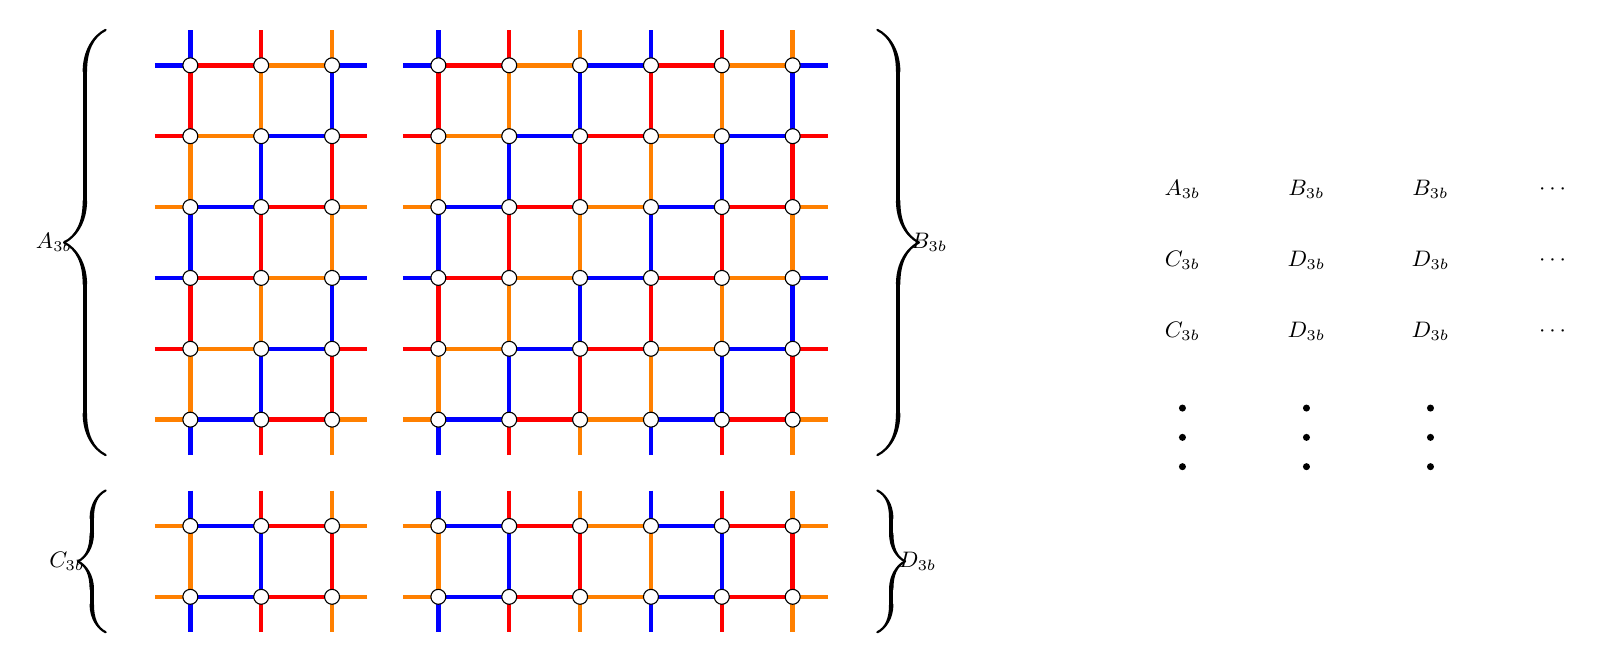
\begin{tikzpicture}[scale=.9, transform shape]
%A Block
    \draw[red, ultra thick] (-.5, -1) -- (0, -1) -- (0, 0) -- (1, 0) -- (1, .5); \draw[red, ultra thick] (-.5, -4) -- (0, -4) -- (0, -3) -- (1, -3) -- (1, -2) -- (2, -2) -- (2, -1) -- (2.5, -1); \draw[red, ultra thick] (1, -5.5) -- (1, -5) -- (2, -5) -- (2, -4) -- (2.5, -4); 
    \draw[blue, ultra thick] (-.5, 0) -- (0, 0) -- (0, .5); \draw[blue, ultra thick] (-.5, -3) -- (0, -3) -- (0, -2) -- (1, -2) -- (1, -1) -- (2, -1) -- (2, 0) -- (2.5,0); \draw[blue, ultra thick] (0, -5.5) -- (0, -5) -- (1, -5) -- (1, -4) -- (2, -4) -- (2, -3) -- (2.5, -3);
    \draw[orange, ultra thick] (-.5, -2) -- (0, -2) -- (0, -1) -- (1, -1) -- (1, 0) -- (2, 0) -- (2, .5); \draw[orange, ultra thick] (-.5, -5) -- (0, -5) -- (0, -4) -- (1, -4) -- (1, -3) -- (2, -3) -- (2, -2) -- (2.5, -2); \draw[orange, ultra thick] (2, -5.5) -- (2, -5) -- (2.5, -5);
    \foreach \x in {0, 1, 2}{\foreach \y in {0, -1, ..., -5}{\draw[draw = black, fill = white] (\x, \y) circle (3pt);}}\draw [ultra thick, decorate, decoration = {calligraphic brace, raise=5pt, amplitude=15pt}] (-1, -5.5) --  (-1, .5) node[pos=.5, left=15pt, black]{\small{$A_{3b}$}};
%B Block
    \draw[red, ultra thick] (3, -1) -- (3.5, -1) -- (3.5, 0) -- (4.5, 0) -- (4.5, .5); \draw[red, ultra thick] (3, -4) -- (3.5, -4) -- (3.5, -3) -- (4.5, -3) -- (4.5, -2) -- (5.5, -2) -- (5.5, -1) -- (6.5, -1) -- (6.5, 0) -- (7.5, 0) -- (7.5, .5); \draw[red, ultra thick] (4.5, -5.5) -- (4.5, -5) -- (5.5, -5) -- (5.5, -4) -- (6.5, -4) -- (6.5, -3) -- (7.5, -3) -- (7.5, -2) -- (8.5, -2) -- (8.5, -1) -- (9, -1); \draw[red, ultra thick] (7.5, -5.5) -- (7.5, -5) -- (8.5, -5) -- (8.5, -4) -- (9, -4);
    \draw[blue, ultra thick] (3, 0) -- (3.5, 0) -- (3.5, .5); \draw[blue, ultra thick] (3, -3) -- (3.5, -3) -- (3.5, -2) -- (4.5, -2) -- (4.5, -1) -- (5.5, -1) -- (5.5, 0) -- (6.5, 0) -- (6.5, .5); \draw[blue, ultra thick] (3.5, -5.5) -- (3.5, -5) -- (4.5, -5) -- (4.5, -4) -- (5.5, -4) -- (5.5, -3) -- (6.5, -3) -- (6.5, -2) -- (7.5, -2) -- (7.5, -1) -- (8.5, -1) -- (8.5, 0) -- (9, 0);\draw[blue, ultra thick] (6.5, -5.5) -- (6.5, -5) -- (7.5, -5) -- (7.5, -4) -- (8.5, -4) -- (8.5, -3) -- (9, -3);
    \draw[orange, ultra thick] (3, -2) -- (3.5, -2) -- (3.5, -1) -- (4.5, -1) -- (4.5, 0) -- (5.5, 0) -- (5.5, .5); \draw[orange, ultra thick] (3, -5) -- (3.5, -5) -- (3.5, -4) -- (4.5, -4) -- (4.5, -3) -- (5.5, -3) -- (5.5, -2) -- (6.5, -2) -- (6.5, -1) -- (7.5, -1) -- (7.5, 0) -- (8.5, 0) -- (8.5, .5); \draw[orange, ultra thick] (5.5, -5.5) -- (5.5, -5) -- (6.5, -5) -- (6.5, -4) -- (7.5, -4) -- (7.5, -3) -- (8.5, -3) -- (8.5, -2) -- (9, -2); \draw[orange, ultra thick] (8.5, -5.5) -- (8.5, -5) -- (9, -5);
    \foreach \x in {3.5, 4.5, 5.5, 6.5, 7.5, 8.5}{\foreach \y in {0, -1, ..., -5}{\draw[draw = black, fill = white] (\x, \y) circle (3pt);}}\draw [ultra thick, decorate, decoration = {calligraphic brace, raise=5pt, amplitude=15pt}] (9.5, .5) --  (9.5, -5.5) node[pos=.5, right=15pt, black]{\small{$B_{3b}$}};
%C Block
    \draw[blue, ultra thick] (0, -6) -- (0, -6.5) -- (1, -6.5) -- (1, -7.5) -- (0, -7.5) -- (0, -8); \draw[red, ultra thick] (1, -6) -- (1, -6.5) -- (2, -6.5) -- (2, -7.5) -- (1, -7.5) -- (1, -8); \draw[orange, ultra thick] (-.5, -6.5) -- (0, -6.5) -- (0, -7.5) -- (-.5, -7.5); \draw[orange, ultra thick] (2, -6) -- (2, -6.5) -- (2.5, -6.5); \draw[orange, ultra thick] (2.5, -7.5) -- (2, -7.5) -- (2, -8); \foreach \x in {0, 1, 2}{\foreach \y in {-6.5, -7.5}{\draw[draw = black, fill = white] (\x, \y) circle (3pt);}}\draw [ultra thick, decorate, decoration = {calligraphic brace, raise=5pt, amplitude=10pt}] (-1, -8) --  (-1, -6) node[pos=.5, left=10pt, black]{\small{$C_{3b}$}};
%D Block
    \draw[blue, ultra thick] (3.5, -6) -- (3.5, -6.5) -- (4.5, -6.5) -- (4.5, -7.5) -- (3.5, -7.5) -- (3.5, -8); \draw[blue, ultra thick] (6.5, -6) -- (6.5, -6.5) -- (7.5, -6.5) -- (7.5, -7.5) -- (6.5, -7.5) -- (6.5, -8); \draw[red, ultra thick] (4.5, -6) -- (4.5, -6.5) -- (5.5, -6.5) -- (5.5, -7.5) -- (4.5, -7.5) -- (4.5, -8); \draw[red, ultra thick] (7.5, -6) -- (7.5, -6.5) -- (8.5, -6.5) -- (8.5, -7.5) -- (7.5, -7.5) -- (7.5, -8); \draw[orange, ultra thick] (5.5, -6) -- (5.5, -6.5) -- (6.5, -6.5) -- (6.5, -7.5) -- (5.5, -7.5) -- (5.5, -8); \draw[orange, ultra thick] (3, -6.5) -- (3.5, -6.5) -- (3.5, -7.5) -- (3, -7.5); \draw[orange, ultra thick] (8.5, -6) -- (8.5, -6.5) -- (9, -6.5); \draw[orange, ultra thick] (9, -7.5) -- (8.5, -7.5) -- (8.5, -8); \foreach \x in {3.5, 4.5, 5.5, 6.5, 7.5, 8.5}{\foreach \y in {-6.5, -7.5}{\draw[draw = black, fill = white] (\x, \y) circle (3pt);}}\draw [ultra thick, decorate, decoration = {calligraphic brace, raise=5pt, amplitude=10pt}] (9.5, -6) --  (9.5, -8) node[pos=.5, right=10pt, black]{\small{$D_{3b}$}};
%Table
    \small{\node at (14, -1.75){$A_{3b}$}; \node at (14, -2.75){$C_{3b}$}; \node at (14, -3.75){$C_{3b}$}; \vvdots{14}{-5.25}; \node at (15.75, -1.75){$B_{3b}$}; \node at (15.75, -2.75){$D_{3b}$}; \vvdots{15.75}{-5.25}; \node at (15.75, -3.75){$D_{3b}$}; \node at (17.5, -1.75){$B_{3b}$}; \node at (17.5, -2.75){$D_{3b}$}; \node at (17.5, -3.75){$D_{3b}$}; \vvdots{17.5}{-5.25};} \node at (19.25, -1.75){$\cdots$}; \node at (19.25, -2.75){$\cdots$}; \node at (19.25, -3.75){$\cdots$};
\end{tikzpicture}\end{center}
}

    
    \column{0.25}
    \block{Decomposing into $C_6$}{
    
    \begin{theorem}
    The graph $C_m \sq C_n$ can be decomposed into copies of $C_6$ if and only if  $m=n=3$, or $n=6$ and $4 \mid m$.
    \end{theorem}
    \\
  \textbf{Example:} \\
  Left: The blue edges cannot be a part of $C_6$. \\
  Right: $C_4 \sq C_6$ decomposed into copies of $C_6$.
  
  \vspace{.2in}
    
  \begin{center}
        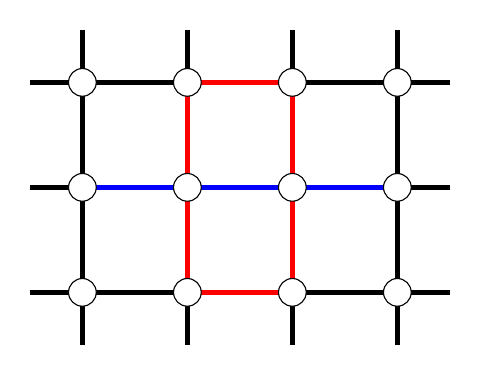
\begin{tikzpicture}
            \foreach \i in {0.5,3.5}{
                \draw [ultra thick, -] (\i*4/3, 0.5*4/3) -- (\i*4/3, 2.5*4/3);
            }
            \foreach \i in {0.5,1.5,...,3.5}{
                \draw [ultra thick, -] (\i*4/3, 0) -- (\i*4/3, 0.5*4/3);
                \draw [ultra thick, -] (\i*4/3, 2.5*4/3) -- (\i*4/3, 3*4/3);
            }
            \foreach \j in {0.5,1.5,2.5}{
                \draw [ultra thick, -] (0*4/3,\j*4/3) -- (0.5*4/3, \j*4/3);
                \draw [ultra thick, -] (4*4/3,\j*4/3) -- (3.5*4/3, \j*4/3);
            }
            \foreach \i in {0.5*4/3, 2.5*4/3}{\foreach \j in {0.5*4/3, 2.5*4/3}{
                \draw [ultra thick, -] (\i,\j) -- (\i+4/3, \j);
            }}
            \draw [ultra thick, -, color=blue] (0.5*4/3, 1.5*4/3) -- (3.5*4/3, 1.5*4/3);
            \draw [ultra thick, -, color=red] (1.5*4/3, 0.5*4/3) -- (2.5*4/3, 0.5*4/3) -- (2.5*4/3, 2.5*4/3) -- (1.5*4/3, 2.5*4/3) -- (1.5*4/3, 0.5*4/3);
            
            \foreach \i in {0.5,1.5,...,3.5}{\foreach \j in {0.5,1.5,2.5}{\filldraw[fill=white, draw=black] (\i*4/3, \j*4/3) circle (5pt);}}
            \end{tikzpicture}
            \hspace{2cm}
            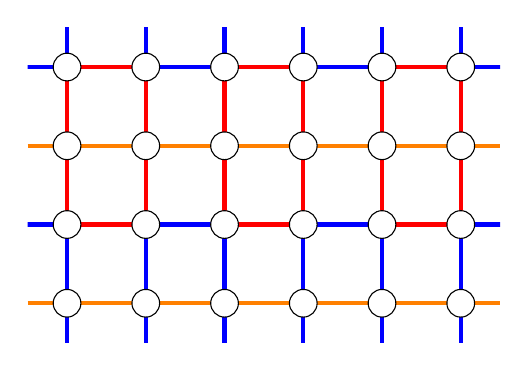
\begin{tikzpicture}
            
            \clip (6.5+3,0) rectangle (12.5+3,4);
            
            \foreach \i in {7,9,11}{
                \draw [ultra thick, -, color=red] (\i+3,3.5) -- (\i+3,1.5) -- (\i+1+3, 1.5) -- (\i+1+3, 3.5) -- (\i+3,3.5);
            }
            \foreach \i in {6,8,10,12}{\foreach \j in {1.5,5.5}{
                \draw [ultra thick, -, color=blue] (\i+3, \j) -- (\i+3, \j-2) -- (\i+1+3,\j-2) -- (\i+1+3,\j) -- (\i+3,\j);
            }}
            \foreach \j in {0.5,2.5}{
                \draw [ultra thick, -, color=orange] (6.5+3,\j) -- (12.5+3,\j);
            }
            
            \foreach \i in {7,8,...,12}{\foreach \j in {0.5,1.5,...,3.5}{\filldraw[fill=white, draw=black] (\i+3, \j) circle (5pt);}}
        \end{tikzpicture}
    \end{center}
     } 
    \block{``Wrapping'' and Odd Cycles}{
      \begin{theorem}
    If $C_k$ decomposes the graph $C_m \sq C_n$, then \[k = 2\ell +mp + nq\] for $p,q \in \mathbb{N}$.
    \end{theorem}
    For a given cycle, we interpret $p$ to be the number of times the cycle ``wraps around'' the torus vertically and $q$ the number of times the cycle wraps around the torus horizontally.
    
    
    \textbf{Example}: $C_4 \sq C_6$ decomposed into copies of $C_{16}$.
    
    \begin{center}
        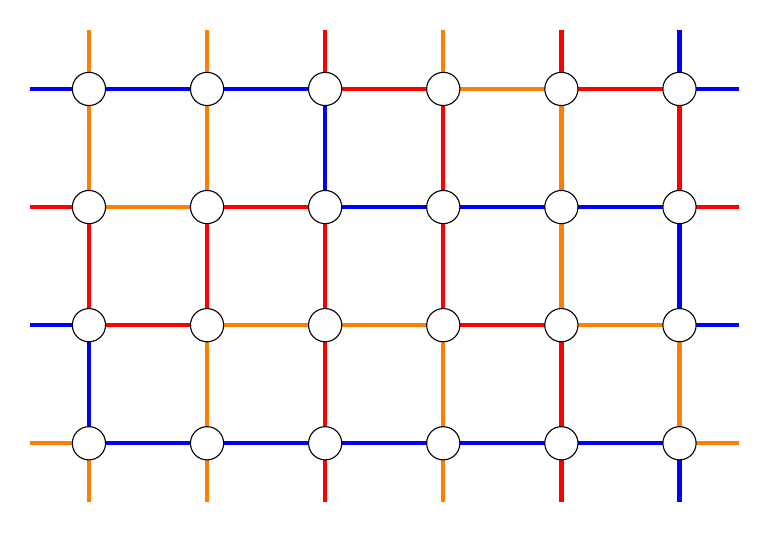
\begin{tikzpicture}[scale=1.5]
            \draw [ultra thick, -, color=red] (-0.5, 2) -- (0, 2) -- (0, 1) -- (1, 1) -- (1, 2) -- (2,2) -- (2, -0.5);
            \draw [ultra thick, -, color=red] (2, 3.5) -- (2,3) -- (3,3) -- (3,1) -- (4,1) -- (4,-0.5);
            \draw [ultra thick, -, color=red] (4, 3.5) -- (4,3) -- (5,3) -- (5,2) -- (5.5, 2);
        
            \draw [ultra thick, -, color=blue] (-0.5, 3) -- (2, 3) -- (2, 2) -- (5,2) -- (5,1) -- (5.5,1);
            \draw [ultra thick, -, color=blue] (-0.5, 1) -- (0, 1) -- (0,0) -- (5,0) -- (5, -0.5);
            \draw [ultra thick, -, color=blue] (5, 3.5) -- (5,3) -- (5.5, 3);
        
            \draw [ultra thick, -, color=orange] (0,3.5) -- (0, 2) -- (1,2) -- (1, 3.5);
            \draw [ultra thick, -, color=orange] (1, -0.5) -- (1,1) -- (3,1) -- (3, -0.5);
            \draw [ultra thick, -, color=orange] (3,3.5) -- (3,3) -- (4,3) -- (4,1) -- (5,1) -- (5,0) -- (5.5, 0);
            \draw [ultra thick, -, color=orange] (-0.5, 0) -- (0,0) -- (0,-0.5);
        
            \foreach \i in {0,1,...,5}{\foreach \j in {0,1,2,3}{\filldraw[fill=white, draw=black] (\i, \j) circle (4pt);}}
            \end{tikzpicture}
            %\small{\node at (16, -1.75){$A_4$}; \node at (17.75, -1.75){$B_4$}; \node at (19.5, -1.75){$B_4$};} \node at (21.25, -1.75){$\cdots$};
            \hspace{0.5cm}
            \begin{tikzpicture}
            \node at (10,3.5) {Color};
            \node at (13,3.5) {$\ell$};
            \node at (15,3.5) {$p$};
            \node at (17,3.5) {$q$};
            \node at (10,2) {Blue};
            \node at (10,0.5) {Red};
            \node at (10,-1) {Orange};
            \node at (13,2) {$0$};
            \node at (15,2) {$1$};
            \node at (17,2) {$2$};
            \node at (13,0.5) {$1$};
            \node at (15,0.5) {$2$};
            \node at (17,0.5) {$1$};
            \node at (15,-1) {$1$};
            \node at (17,-1) {$1$};
            \node at (13,-1) {$3$};
            
            \draw [thick, -] (8.5,2.75) -- (17.5,2.75);
            \draw [thick, -] (12, 4) -- (12,-2);
        \end{tikzpicture}
    \end{center}
    
    \begin{theorem}
        If $k$ is odd and $m, n > k$, then $C_k$ does not decompose $C_m \sq C_n$.
    \end{theorem}
    
    \begin{theorem}
        If $n$ and $m$ are odd and $n < 2m$, then $C_n$ decomposes $C_m \sq C_n$.
    \end{theorem}
    
    \textbf{Example: } $C_{9}$ decomposing $C_7 \sq C_9$ (left) and $C_{11}$ decomposing $C_7 \sq C_{11}$ (right).
    
      \vspace{.2in}


    \begin{center}
        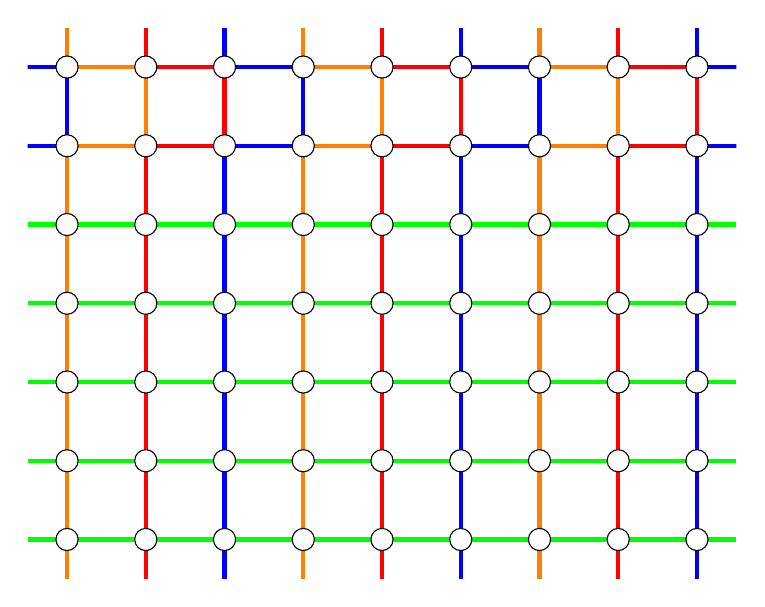
\begin{tikzpicture}
        %\small{\node at (3.25,-1) {$C_9$ decomposing $C_7 \sq C_9$.};}
        \begin{scope}
            \clip (-0.5, -0.5) rectangle (8.5,6.5);
            
            \foreach \i\j in {-1/blue, 0/orange, 1/red, 2/blue, 3/orange, 4/red, 5/blue, 6/orange, 7/red, 8/blue, 9/orange}{
                \draw [ultra thick, -, color=\j] (\i, -0.5) -- (\i, 5) -- (\i+1, 5) -- (\i+1, 6) -- (\i, 6) -- (\i, 6.5);
            }
            \foreach \j in {0,1,...,4}{
                \draw [ultra thick, -, color=green] (-0.5, \j) -- (8.5, \j);
            }
          
            \foreach \i in {0,1,...,8}{\foreach \j in {0,1,...,6}{
                \filldraw[fill=white, draw=black] (\i, \j) circle (4pt);
            }}
        \end{scope}
        \end{tikzpicture}
        \hspace{0.5in}
        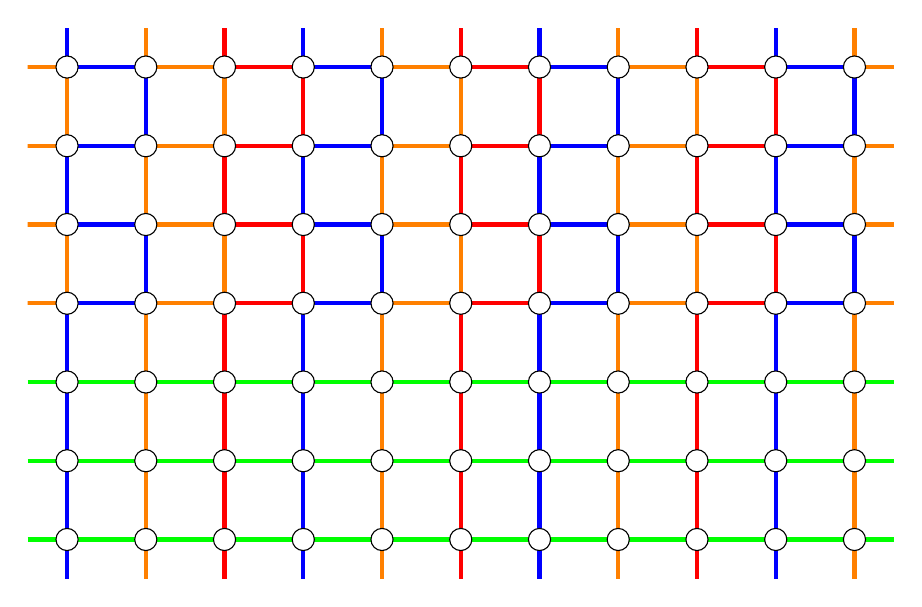
\begin{tikzpicture}
        %\small{\node at (13.5,-1) {$C_{11}$ decomposing $C_7 \sq C_{11}$.};}
        \begin{scope}
            \clip (9.5,-0.5) rectangle (20.5,6.5);
            
            \foreach \i\j in {9/orange, 10/blue, 11/orange, 12/red, 13/blue, 14/orange, 15/red, 16/blue, 17/orange, 18/red, 19/blue, 20/orange}{
                \draw [ultra thick, -, color=\j] (\i, -0.5) -- (\i, 3) -- (\i+1, 3) -- (\i+1,4) -- (\i,4) -- (\i,5) -- (\i+1, 5) -- (\i+1, 6) -- (\i,6) -- (\i,6.5);
            }
            
            \foreach \j in {0,1,2}{
                \draw [ultra thick, -, color=green] (9.5,\j) -- (20.5,\j);
            }
            
            \foreach \i in {10,11,...,20}{\foreach \j in {0,1,...,6}{
                \filldraw[fill=white, draw=black] (\i, \j) circle (4pt);
            }}
        \end{scope}
        \end{tikzpicture}
    \end{center}
    
}
    \block{References \& Acknowledgements}{\small
    \fullcite{gibson_offner} \\
    \fullcite{kotzig}\\}
     


\end{columns}


\end{document}
